%%%%%%%%%%%%%%%%%%%%%%%%%%%%%%%%%%%%%%%%%%%%%%%%%%%%%%%%%%%%%%%%%%%%%%
% Lớp 12 | Nguyên hàm, tích phân | Tích phân
% Dạng 2D4?2-2: Tích phân cơ bản đa thức, phân thức
% Số câu: 92  (sinh tự động bởi tach_cau.py; từ nay thầy sửa trực tiếp file này)
%%%%%%%%%%%%%%%%%%%%%%%%%%%%%%%%%%%%%%%%%%%%%%%%%%%%%%%%%%%%%%%%%%%%%%

%%%%%%%%%%%%%%%% TRẮC NGHIỆM 4 PHƯƠNG ÁN %%%%%%%%%%%%%%%%

% nguồn: Phan1_Lop_12_Dai_so_Chuong_4
\begin{ex}%[2D4N2-2]%[ma:21c7796e]
	Tích phân $\displaystyle\int_1^52x\mathrm{\,d}x$  bằng
	\choice 
		{$4$} 
		 {\True $24$}
		 {$21$}
		{$6$} 
	 \loigiai{
		 Ta có $\displaystyle\int_1^52x\mathrm{\,d}x = \dfrac{2x^2}{2}\Big|_{1}^{5} = x^2\Big|_{1}^{5} = 5^2 - 1^2 = 24$.
	} 
\end{ex}

% nguồn: Phan1_Lop_12_Dai_so_Chuong_4
\begin{ex}%[2D4N2-2]%[ma:dec0231e]
	Tích phân $I = \displaystyle\int_0^1  \left(3x^2 + 2x\right)\mathrm{d}x$ bằng
	 \choice
		{$0$} 
		 {$4$}
		 {\True $2$}
		 {$-6$}
	\loigiai{$I = \displaystyle\int_0^1 (3x^2 + 2x) \mathrm{d}x = \left(x^3 + x^2\right)\big|_0^1 = (1  + 1)-(0+0) = 2$.
	} 
\end{ex}

% nguồn: Phan1_Lop_12_Dai_so_Chuong_4
\begin{ex}%[2D4N2-2]%[ma:34820a90]
	Tích  phân $I=\displaystyle\int_{-1}^1\left(x^3+3 x+2\right)\mathrm{\,d}x$ có giá trị là
	 \choice
		 {\True $I=4$}
		 {$I=2$}
		{$I=3$} 
		 {$I=1$}
	 \loigiai{$I=\displaystyle\int_{-1}^1\left(x^3+3 x+2\right)\mathrm{\,d}x=4$.}
\end{ex}

% nguồn: Phan1_Lop_12_Dai_so_Chuong_4
\begin{ex}%[2D4N2-2]%[ma:05f1dcae]
	Tính tích phân  $I=\displaystyle\int_0^2 (2x+1)\mathrm{\,d}x$.
	\choice 
		 {$I=4$}
		 {$I=5$}
		 {\True $I=6$}
		 {$I=2$}
	 \loigiai{
	Ta có  $I=\displaystyle\int_0^2 (2x+1)\mathrm{\,d}x=6$.
	 }
\end{ex}

% nguồn: Phan1_Lop_12_Dai_so_Chuong_4
\begin{ex}%[2D4N2-2]%[ma:5978a759]
	 Tích phân $\displaystyle\int_{2}^{3}2xdx$ bằng
	 \choice
		 {\True $3$}
		 {$2$}
		 {$1$}
		{$4$} 
	 \loigiai{
	Ta có $\displaystyle\int_{2}^{3}2xdx = x^2\Big|_2^3  = 3^2 - 2^2 = 3$.}
\end{ex}

% nguồn: Phan1_Lop_12_Dai_so_Chuong_4
\begin{ex}%[2D4N2-2]%[ma:4348c048]
	Khẳng định  nào dưới đây đúng?
	 \choice
		{$\displaystyle\int x^3\,\mathrm{d}x  = x^3 + C$}
		{\True $\displaystyle\int x^3\,\mathrm{d}x = \dfrac{1}{4}x^4 + C$} 
		{$\displaystyle\int x^3\,\mathrm{d}x =  \dfrac{3}{4}x^4 + C$}
		 {$\displaystyle\int x^3\,\mathrm{d}x = \dfrac{2}{3}x^3 + C$}
	 \loigiai{
	 }
\end{ex}

% nguồn: Phan1_Lop_12_Dai_so_Chuong_4
\begin{ex}%[2D4N2-2]%[ma:67fc3a81]
	Nếu $\displaystyle\int_1^3 f(x)\,\mathrm{d}x = 2$ thì  $\displaystyle\int_1^3\left[f(x) + 2x\right]\,\mathrm{d}x$ bằng
	 \choice
		 {$20$}
		 {\True $10$}
		 {$12$}
		 {$18$}
	\loigiai{ 
		Ta có $\displaystyle\int_1^3\left[f(x) + 2x\right]\,\mathrm{d}x = \displaystyle\int_1^3f(x) \,\mathrm{d}x+ \displaystyle\int_1^3 2x \,\mathrm{d}x  = 2+8=10$.
	 }
\end{ex}

% nguồn: Phan1_Lop_12_Dai_so_Chuong_4
\begin{ex}%[2D4N2-2]%[ma:b997c0d6]
	Họ các nguyên hàm của hàm số $f(x)=3x^2-4x$  là
	\choice 
		{$F(x)=6x-4+C$} 
		{$F(x)=x^3+2x^2+C$} 
		 {\True$F(x)=x^3-2x^2+C$}
		 {$F(x)=x^3-4+C$}
	\loigiai{Ta có $f(x)=\displaystyle \int f(x)\mathrm{\,d}x=\displaystyle \int \left(3x^2-4x\right)\mathrm{\,d}x=x^3-2x^2+C$.} 
\end{ex}

% nguồn: Phan1_Lop_12_Dai_so_Chuong_4
\begin{ex}%[2D4H2-2]%[ma:3c1aed4a]
	Cho $\displaystyle\int_{-1}^2{f(x)\mathrm{\,d}x}=3$, $\displaystyle\int_{-1}^2{g(x)\mathrm{\,d}x}=-1$.  Khi đó $I=\displaystyle\int_{-1}^2{\left[x+2f(x)-3g(x)\right]\mathrm{\,d}x}$ bằng
	\choice 
		{$10$} 
		{\True $\dfrac{21}2$} 
		{$\dfrac{19}2$} 
		{$\dfrac{17}2$} 
	\loigiai{ 
		Ta  có \[I=\displaystyle\int_{-1}^2{\left[x+2f(x)-3g(x)\right]\mathrm{\,d}x}=\displaystyle\int_{-1}^2{x\mathrm{\,d}x}+2\displaystyle\int_{-1}^2{f(x)\mathrm{\,d}x}-3\displaystyle\int_{-1}^2{g(x)\mathrm{\,d}x}=\dfrac32+2\cdot3-3\cdot\left(-1\right)=\dfrac{21}2.\]
	} 
\end{ex}

% nguồn: Phan1_Lop_12_Dai_so_Chuong_4
\begin{ex}%[2D4H2-2]%[ma:86bab69c]
	Nếu $\displaystyle\int_{1}^{3} f(x) \mathrm{\,d}x =2$ thì $\displaystyle\int_{1}^{3}[f(x)+2x] \mathrm{\,d}x $  bằng
	 \choice
		{$18$} 
		 {\True $10$}
		{$12$} 
		 {$20$}
	 \loigiai{
		$\displaystyle\int_1^3[f(x)+2 x] \mathrm{\,d}x =\displaystyle\int_{1}^{3}f(x)\mathrm{\,d}x +2\displaystyle\int_{1}^{3}x \mathrm{\,d}x =2+2\cdot 4=10$. 
	} 
\end{ex}

% nguồn: Phan1_Lop_12_Dai_so_Chuong_4
\begin{ex}%[2D4H2-2]%[ma:032e39eb]
	Cho hàm số $y=f(x)$ liên tục trên đoạn $[-6;11]$ và thỏa mãn $\displaystyle\int_{-6}^{11} f(x)\, \mathrm{d}x=8$, $\displaystyle\int_{2}^{6} f(x)\, \mathrm{d}x=3$.  Giá trị của biểu thức $P=\displaystyle\int_{-6}^{2} f(x)\, \mathrm{d}x+\displaystyle\int_{6}^{11} f(x)\, \mathrm{d}x$ bằng
	\choice 
		 {$P=4$}
		{$P=11$} 
		{\True  $P=5$}
		 {$P=2$}
	 \loigiai{
		Ta  có
		$\displaystyle\int_{-6}^{11} f(x)\, \mathrm{d}x=\displaystyle\int_{-6}^{2} f(x)\,  \mathrm{d}x+\displaystyle\int_{2}^{6} f(x)\, \mathrm{d}x+\displaystyle\int_{6}^{11} f(x)\, \mathrm{d}x$.\\
		$\Rightarrow 8=\displaystyle\int_{-6}^{2} f(x)\, \mathrm{d}x+3+\displaystyle\int_{6}^{11}  f(x)\, \mathrm{d}x$.\\
		$P=\displaystyle\int_{-6}^{2} f(x)\, \mathrm{d}x+\displaystyle\int_{6}^{11} f(x)\, \mathrm{d}x=8-3=5$. 
	} 
\end{ex}

% nguồn: Phan1_Lop_12_Dai_so_Chuong_4
\begin{ex}%[2D4H2-2]%[ma:f4361b03]
	Tính $I=\displaystyle\int_0^1{\left(\dfrac1{2x+1}+3\sqrt x\right)}\mathrm{\,d}x$. 
	\choice 
		{\True $2+\ln\sqrt3$} 
		{$4+\ln 3$} 
		{$2+\ln  3$}
		{$1+\ln\sqrt3$} 
	\loigiai{ 
		Ta có  \[I=\displaystyle\int_0^1{\left(\dfrac1{2x+1}+3\sqrt x\right)}\mathrm{\,d}x=\left(\dfrac12\ln|2x+1 |+2x\sqrt x\right) \Bigg|_0^1=\dfrac12\ln 3+2=2+\ln\sqrt3.\]
	 }
\end{ex}

% nguồn: Phan1_Lop_12_Dai_so_Chuong_4
\begin{ex}%[2D4H2-2]%[ma:a6123ca8]
	Biết hàm số $F(x)=x^2$ là một nguyên hàm của hàm số $f(x)$ trên  $\mathbb{R}$. Tích phân $\displaystyle\int_1^2f(x) \mathrm{\,d}x$ bằng
	\choice 
		{$1$} 
		{$-3$} 
		{\True $3$} 
		{$5$} 
	\loigiai{ 
		Ta có $\displaystyle\int_1^2f(x) \mathrm{\,d}x=x^2  \Big |_1^2=3$.
	 }
\end{ex}

% nguồn: Phan1_Lop_12_Dai_so_Chuong_4
\begin{ex}%[2D4H2-2]%[ma:7e306aff]
	 Cho hàm số $f(x)=\heva{&4-x&&\text{ khi }0\leq x\leq 1\\
	&3x^2&&\text{ khi }1\leq x\leq 2}$. Tính tích phân $I=\int_0^2f(x)\mathrm{\,d}x$. 
	 \choice
		 {\True $\dfrac{21}{2}$}
		{$\dfrac{7}{2}$} 
		 {$7$}
		 {$\dfrac{5}{2}$}
	 \loigiai{
		Ta  có $I=\int_0^2f(x)\mathrm{\,d}x=\int_0^1f(x)\mathrm{\,d}x+\int_1^2f(x)\mathrm{\,d}x=\int_0^1(4-x)\mathrm{\,d}x+\int_1^23x^2\mathrm{\,d}x=\dfrac{21}{2}$.
	 }
\end{ex}

% nguồn: Phan1_Lop_12_Dai_so_Chuong_4
\begin{ex}%[2D4H2-2]%[ma:2edc6243]
	Tính $I=\displaystyle \int_0^1 \left( \mathrm{e}^x +3\sqrt{x} \right) \mathrm{\,d}x$. 
	 \choice
		 {$2+\mathrm{e}$}
		{$1+\mathrm{e}$} 
		 {$1+\mathrm{e}^2$}
		 {$3$}
	 \loigiai{
		Ta có $I=\displaystyle\int_0^1 \left( \mathrm{e}^x +3\sqrt{x} \right) \mathrm{\,d}x = \left( \mathrm{e}^x +  2x\sqrt{x} \right) \Big|_0^1 = \mathrm{e}+2$.
	} 
\end{ex}

% nguồn: Phan1_Lop_12_Dai_so_Chuong_4
\begin{ex}%[2D4H2-2]%[ma:255860af]
	Nếu $\displaystyle\int_0^1{2f(x)\mathrm{\,d}x=6}$ thì  $\displaystyle\int_0^1{\left[\dfrac13f(x)+2x\right]\mathrm{\,d}x}$ bằng
	 \choice
		{$4$} 
		 {$7$}
		{$3$} 
		{\True  $2$}
	 \loigiai{
		Ta  có \[\displaystyle\int_0^1{\left[\dfrac13f(x)+2x\right]\mathrm{\,d}x}=\dfrac13\displaystyle\int_0^1{f(x)\mathrm{\,d}x}+2\displaystyle\int_0^1{x\mathrm{\,d}x}=\dfrac16\displaystyle\int_0^1{2f(x)\mathrm{\,d}x}+ {x^2} \Bigg|_0^1=\dfrac16\cdot6+1=2.\]
	 }
\end{ex}

% nguồn: Phan1_Lop_12_Dai_so_Chuong_4
\begin{ex}%[2D4H2-2]%[ma:96f5c22f]
	Nếu $\displaystyle\int_0^2f(x)\,\mathrm{d}x=3$ thì $\displaystyle\int_0^2[2x-f(x)]\,\mathrm{d}x$ bằng 
	\choice 
		{$7$} 
		 {$10$}
		 {\True $1$}
		{$-2$} 
	 \loigiai{Ta có $\displaystyle\int_0^2[2x-f(x)]\,\mathrm{d}x
		 =\displaystyle\int_0^22x\,\mathrm{d}x
		-\displaystyle\int_0^2f(x)\,\mathrm{d}x 
		=x^2\Bigg|_0^2-3 
		=4-3 
		 =1
	 $.}
\end{ex}

% nguồn: Phan1_Lop_12_Dai_so_Chuong_4
\begin{ex}%[2D4H2-2]%[ma:45ee09b5]
	Nếu  $\displaystyle\int_1^4{f(x)} \mathrm{\,d}x=-2$ và $\displaystyle\int_1^4{g(x)} \mathrm{\,d}x=-6$ thì $\displaystyle\int_1^4{\left[2f(x)-g(x)+1\right]} \mathrm{\,d}x$ bằng
	\choice 
		 {$2$}
		{$-4$} 
		{\True  $5$}
		{$3$} 
	 \loigiai{
		Ta  có \[\displaystyle\int_1^4{\left[2f(x)-g(x)+1\right]} \mathrm{\,d}x=2\displaystyle\int_1^4{f(x)} \mathrm{\,d}x-\displaystyle\int_1^4{g(x)} \mathrm{\,d}x+\displaystyle\int_1^41 \mathrm{\,d}x=2\cdot(-2)+6+3=5.\]
	} 
\end{ex}

% nguồn: Phan1_Lop_12_Dai_so_Chuong_4
\begin{ex}%[2D4H2-2]%[ma:736793e2]
	Tính tích  phân $\displaystyle\int_0^1(2\,024x+2\,025)\,\mathrm{d}x$.
	\choice 
		{$4\,049$} 
		{$-3\,037$} 
		{\True  $3\,037$}
		 {$-4\,049$}
	\loigiai{Ta  có $\displaystyle\int_0^1(2\,024x+2\,025)\,\mathrm{d}x
	 =\left(1\,012x^2+2\,025x\right) \Bigg|_0^1=1\,012+2\,025=3\,037$.}
\end{ex}

% nguồn: Phan1_Lop_12_Dai_so_Chuong_4
\begin{ex}%[2D4H2-2]%[ma:3db3a697]
	Tích phân  $I=\displaystyle\int_0^1{\dfrac1{x+2}\mathrm{\,d}x}$ bằng
	\choice 
		 {$-\ln 3$}
		{$\ln 3$} 
		{$1-\ln  3$}
		{\True $\ln 3-\ln 2$} 
	\loigiai{Ta có $I=\displaystyle\int_0^1{\dfrac1{x+2}\mathrm{\,d}x}=\ln|x+2 |\Bigg|_0^1=\ln  3-\ln 2$.}
\end{ex}

% nguồn: Phan1_Lop_12_Dai_so_Chuong_4
\begin{ex}%[2D4H2-2]%[ma:db7ca8ba]
	Cho $\displaystyle\int_{-1}^2{f\left(t\right)} \mathrm{\,d}t=2$ và$\displaystyle\int_{-1}^2{g(x)}\mathrm{\,d}x=-1$. Tính  $I=\displaystyle\int_{-1}^2{\left[x+2f(x)-3g(x)\right]}\mathrm{\,d}x$.
	 \choice
		 {\True $I=\dfrac{17}2$}
		{$I=\dfrac72$} 
		{$I=\dfrac52$} 
		{$I=\dfrac{11}2$} 
	\loigiai{ 
		Ta có  \[I=\displaystyle\int_{-1}^2{\left[x+2f(x)-3g(x)\right]}\mathrm{\,d}x=\displaystyle\int_{-1}^2x\mathrm{\,d}x+2\displaystyle\int_{-1}^2{f(x)}\mathrm{\,d}x-3\displaystyle\int_{-1}^2{g(x)}\mathrm{\,d}x=\dfrac32+2\cdot2-3\left(-1\right)=\dfrac{17}2.\]
	} 
\end{ex}

% nguồn: Phan1_Lop_12_Dai_so_Chuong_4
\begin{ex}%[2D4H2-2]%[ma:1960c318]
	Nếu $\displaystyle\int_0^4f(x)\mathrm{\,d}x=37$  thì $\displaystyle\int_0^4\left[2f(x)-3x^2\right]\mathrm{\,d}x$ bằng
	\choice 
		 {$-27$}
		 {$18$}
		 {$12$}
		{\True $10$} 
	\loigiai{$\displaystyle\int_0^4\left[2f(x)-3x^2\right]\mathrm{\,d}x=2\displaystyle\int_0^4 f(x)\mathrm{\,d}x-\displaystyle\int_0^4 3x^2 \mathrm{\,d}x =2 \cdot 37 - 64=10$.} 
\end{ex}

% nguồn: Phan1_Lop_12_Dai_so_Chuong_4
\begin{ex}%[2D4H2-2]%[ma:3422246c]
	Cho hàm số $f(x)=\heva{&3x^2&&\text{ khi }0\leq x\leq 1\\ 
	&4-x&&\text{  khi }1\leq x\leq 2}$. Tính tích phân $\displaystyle\int_0^2f(x)\mathrm{\,d}x$.
	 \choice
		 {\True $\dfrac{7}{2}$}
		{$1$} 
		 {$\dfrac{5}{2}$}
		 {$\dfrac{3}{2}$}
	\loigiai{ 
		Ta  có $\displaystyle\int_0^2f(x)\mathrm{\,d}x=\int_0^1f(x)\mathrm{\,d}x+\int_1^2f(x)\mathrm{\,d}x=\int_0^13x^2\mathrm{\,d}x+\int_1^2(4-x)\mathrm{\,d}x=1+\dfrac{5}{2}=\dfrac{7}{2}$.
	} 
\end{ex}

% nguồn: Phan1_Lop_12_Dai_so_Chuong_4
\begin{ex}%[2D4H2-2]%[ma:b1db1d85]
	Cho $\displaystyle\int_{2}^{3}f(x)dx = 1$ và $\displaystyle\int_{2}^{3}g(x)dx=4$. Khi đó $\displaystyle\int_{2}^{3}[f(x)+g(x)]dx$  bằng
	\choice 
		 {\True $5$}
		{$3$} 
		{$-3$} 
		{$4$} 
	\loigiai{ 
	Ta  có $\displaystyle\int_{2}^{3}[f(x)+g(x)]dx= \displaystyle\int_{2}^{3}f(x)dx+\displaystyle\int_{2}^{3}g(x)dx=1+4=5$.}
\end{ex}

% nguồn: Phan1_Lop_12_Dai_so_Chuong_4
\begin{ex}%[2D4H2-2]%[ma:18b55b32]
	Nếu $b-a=3$ thì  biểu thức $\displaystyle\int_a^b x^2\mathrm{\,d}x$ có giá trị bằng
	\choice 
		 {$3-ab$}
		 {$9-3ab$}
		{\True  $9+3ab$}
		{$3+ab$} 
	 \loigiai{
		 $\displaystyle\int_a^b x^2\mathrm{\,d}x = \dfrac{x^3}{3} \bigg|_a^b = \dfrac{b^3 - a^3}{3} = \dfrac{(b-a)\left(b^2+ab+a^2\right)}{3}= (b-a)^2+3ab = 9+3ab$.
	 }
\end{ex}

% nguồn: Phan1_Lop_12_Dai_so_Chuong_4
\begin{ex}%[2D4H2-2]%[ma:94a2f84a]
	Cho $\displaystyle\int_{0}^{1}  f(x)\mathrm{\,d}x=1$. Tích phân $\displaystyle\int_{0}^{1} \left(2f(x)-3x^2\right)\mathrm{\,d}x$ bằng
	 \choice
		 {\True $1$}
		{$0$} 
		{$3$} 
		{$-1$} 
	\loigiai{Ta có $\displaystyle\int_{0}^{1} \left(2f(x)-3x^2\right)\mathrm{\,d}x=2\displaystyle\int_{0}^{1} f(x) \mathrm{\,d}x-\displaystyle\int_{0}^{1} 3x^2\mathrm{\,d}x= 2  \cdot 1- 1=1$.}
\end{ex}

% nguồn: Phan1_Lop_12_Dai_so_Chuong_4
\begin{ex}%[2D4H2-2]%[ma:ba4af229]
	Cho $\displaystyle\int_0^2 f(x) \mathrm{\,d}x=2\,026$, tích phân $\displaystyle\int_0^2\left(2f(x)-3x^2\right) \mathrm{\,d}x$  bằng
	\choice 
		{$8\,096$} 
		 {$8\,112$}
		 {\True $4\,044$}
		 {$4\,060 $}
	 \loigiai{
		Ta có  $\displaystyle\int_0^2\left(2 f(x)-3 x^{2}\right) \mathrm{\,d} x=\displaystyle\int_0^2 2f(x)\mathrm{\,d}x-\displaystyle\int_0^2 3x^2 \mathrm{\,d}x=2\displaystyle\int_0^2 f(x)\mathrm{\,d}x-x^3\Bigg|_0^2=2\cdot2\,026-8=4\,044$.
	} 
\end{ex}

% nguồn: Phan1_Lop_12_Dai_so_Chuong_4
\begin{ex}%[2D4H2-2]%[ma:a8cb60e4]
	 [GV:Xuan Vy Pham]
	Cho $\displaystyle\int_{0}^{1} f(x)\mathrm{\,d}x=1$. Tích phân $\displaystyle\int_{0}^{1} \left(2f(x)-3x^2\right)\mathrm{\,d}x$  bằng
	\choice 
		{\True $1$} 
		{$0$} 
		 {$3$}
		{$-1$} 
	\loigiai{Ta có $\displaystyle\int_{0}^{1} \left(2f(x)-3x^2\right)\mathrm{\,d}x=2\displaystyle\int_{0}^{1} f(x) \mathrm{\,d}x-\displaystyle\int_{0}^{1} 3x^2\mathrm{\,d}x=  2 \cdot 1- 1=1$.}
\end{ex}

% nguồn: Phan1_Lop_12_Dai_so_Chuong_4
\begin{ex}%[2D4H2-2]%[ma:1324b474]
	Cho hàm số $f(x)=\heva{&x+2&&\text{ khi }-3\leq x\leq -1\\&x^2\quad&&\text{ khi  }x\geq -1}$ thì $\displaystyle\int_{-3}^3f(x)\mathrm{\,d}x$ bằng
	\choice 
		 {$\dfrac{31}{3}$}
		 {\True $\dfrac{28}{3}$}
		{$\dfrac{22}{3}$} 
		 {$\dfrac{26}{3}$}
	 \loigiai{
		Ta có \allowdisplaybreaks\begin{eqnarray*}
		\int_{-3}^3f(x)\mathrm{\,d}x&=&\int_{-3}^{-1}f(x)\mathrm{\,d}x+\int_{-1}^3f(x)\mathrm{\,d}x\\ 
		&=&\int_{-3}^{-1}(x+2)\mathrm{\,d}x+\int_{-1}^3x^2\mathrm{\,d}x\\ 
		&=&0+\dfrac{28}{3}\\ 
		 &=&\dfrac{28}{3}.
	\end{eqnarray*}
	Vậy  $\displaystyle\int_{-3}^3f(x)\mathrm{\,d}x=\dfrac{28}{3}$.
 }
\end{ex}

% nguồn: Phan1_Lop_12_Dai_so_Chuong_4
\begin{ex}%[2D4H2-2]%[ma:e40c1119]
	 Cho $\displaystyle\int_1^2[2f(x)-3x+1]\mathrm{\,d}x=\dfrac{1}{2}$. Tính $\displaystyle\int_1^2f(x)\mathrm{\,d}x$
	 \choice
		 {$1$}
		 {\True $2$}
		 {$3$}
		{$4$} 
	 \loigiai{Ta có
		\begin{eqnarray*} &&\displaystyle\int_1^2[2f(x)-3x+1] \mathrm{\,d}x=\dfrac{1}{2} \\
			 &\Leftrightarrow & 2\displaystyle\int_1^2 f(x) \mathrm{\,d}x+\displaystyle\int_1^2(-3x+1) \mathrm{\,d}x =\dfrac{1}{2} \\
			&\Leftrightarrow &  2\displaystyle\int_1^2 f(x) \mathrm{\,d}x -\dfrac{7}{2}=\dfrac{1}{2}\\
			 &\Leftrightarrow &\displaystyle\int_1^2f(x)\mathrm{\,d}x=2.
	\end{eqnarray*} }
\end{ex}

% nguồn: Phan1_Lop_12_Dai_so_Chuong_4
\begin{ex}%[2D4H2-2]%[ma:66d4b6a3]
	Biết $F(x)=x^3$ là  một nguyên hàm của hàm số $ f(x)$ trên $\mathbb{R}$. Giá trị của $\displaystyle\int_1^2{\left(2+f(x)\right)\mathrm{\,d}x}$ bằng
	 \choice
		 {$7$}
		{\True  $9$}
		{$\dfrac{15}4$} 
		{$\dfrac{23}4$} 
	 \loigiai{
		 Ta có \[\displaystyle\int_1^2{\left(2+f(x)\right)\mathrm{\,d}x}=\displaystyle\int_1^2{2\mathrm{\,d}x}+\displaystyle\int_1^2{f(x)\mathrm{\,d}x}= 2x \Bigg|_1^2+ {x^3} \Bigg|_1^2=9.\]
	 }
\end{ex}

% nguồn: Phan1_Lop_12_Dai_so_Chuong_4
\begin{ex}%[2D4V2-2]%[ma:708b3f74]
	Cho $a$ là số thực dương, tính tích phân $I=\displaystyle\int_{-1}^a|x|\mathrm{\,d}x$  theo $a$.
	\choice 
		 {\True $I=\dfrac{a^2+1}{2}$}
		 {$I=\dfrac{a^2+2}{2}$}
		 {$I=\dfrac{-2a^2+1}{2}$}
		{$I=\dfrac{\left|3a^2-1\right|}{2}$} 
	 \loigiai{
		Vì $a >  0$ nên $I=-\displaystyle\int_{-1}^0x \mathrm{\,d}x+\int_0^a x \mathrm{\,d}x=\dfrac{1}{2}+\dfrac{a^2}{2}=\dfrac{1+a^2}{2}$.
	} 
\end{ex}

% nguồn: Phan1_Lop_12_Dai_so_Chuong_4
\begin{ex}%[2D4V2-2]%[ma:6d5d50eb]
	 Cho hàm số $y=f(x)=1$, $y=g(x)=|x|$. Giá trị $I=\displaystyle\int_{-1}^2\min \{f(x); g(x)\} \mathrm{\,d}x$ bằng
	\choice 
		 {$1$}
		{$\dfrac{3}{2}$} 
		 {\True $2$}
		{$\dfrac{5}{2}$} 
	 \loigiai{
		Xét bất phương trình $|x|>  1\Leftrightarrow\hoac{&x > 1\\&x <-1.}$\\
		Suy ra $\min \{1;|x|\}=1$ khi $1< x$  hoặc $x <-1$ và $\min \{1;|x|\}=|x|$ khi $-1< x < 1$.\\
		 Ta có
		\begin{eqnarray*}
			I=\int_{-1}^2\min \{1;|x|\} \mathrm{\,d}x&=&\int_{-1}^1\min \{1;|x|\} \mathrm{\,d}x+\int_1^2\min  \{1;|x|\} \mathrm{\,d}x\\
			&=&\int_{-1}^1|x|\mathrm{\,d}x+\int_1^2\mathrm{\,d}x\\ 
			&=&\int_{-1}^0-x \mathrm{\,d}x+\int_0^1x \mathrm{\,d}x+\int_1^2\mathrm{\,d}x\\ 
			&=&\left.\dfrac{-x^2}{2}\right|_{-1}^0+\left.\dfrac{x^2}{2}\right|_0 ^1+x\bigg|_1  ^2\\
			&=&2. 
		\end{eqnarray*}
	} 
\end{ex}

% nguồn: Phan1_Lop_12_Dai_so_Chuong_4
\begin{ex}%[2D4V2-2]%[ma:823a3d65]
	Có bao nhiêu giá trị thực của tham  số $m$ thỏa mãn $\displaystyle\int_0^m\left|3x^2-2x\right|\mathrm{\,d}x=m-10$?
	 \choice
		 {\True $1$}
		{$2$} 
		{$4$} 
		 {$3$}
	\loigiai{ 
		 Đặt $I=\displaystyle\int_0^m\left|3x^2-2x\right|\mathrm{\,d}x=m-10$; $f(x)=3x^2-2x$.\\
		 Dấu của $f(x)$
		\begin{center}
			\begin{tikzpicture}
					\tkzTabInit[lgt=1.2,espcl=2.5,nocadre=true] 
						 {$x$/0.6,$f (x)$/0.6}
						{$-\infty$,$0$,$\tfrac{2}{3}$,$+\infty$} 
					 \tkzTabLine{,+,0,-,0,+,}
				\end{tikzpicture}
		\end{center}
		 Xét các trường hợp sau
		\begin{itemize}
			\item Nếu $m < 0$ thì $I=\displaystyle\int_0^m\left(3x^2-2x\right) \mathrm{\,d}x=\left.\left(x^3-x^2\right)\right|_0  ^m=m^3-m^2=m-10$.\\
			 Suy ra $m^3-m^2-m+10=0\Leftrightarrow m=-2$ (thỏa mãn).
			\item Nếu $0\leq  m < \dfrac{2}{3}$ thì $I=-\displaystyle\int_0^m\left(3x^2-2x\right) \mathrm{\,d}x=-\left.\left(x^3-x^2\right)\right|_0 ^m=-m^3+m^2=m-10$.\\
			Suy ra $m^3-m^2+m-10=0\Leftrightarrow m \approx  2{,}36$. (loại).
			\item Nếu $m \geq \dfrac{2}{3}$ thì 
			\begin{eqnarray*}
				I&=&-\int_0^{\tfrac{2}{3}}\left(3x^2-2x\right)\mathrm{\,d}x+\int_{\tfrac{2}{3}}^m\left(3x^2-2x\right)\mathrm{\,d}x\\ 
				&=&\dfrac{4}{27}+\left(x^3-x^2\right)\bigg|_m^{\tfrac{2}{3}}\\ 
				 &=&m^3-m^2+\dfrac{8}{27}.
			\end{eqnarray*}
			Khi đó  $I=m-10\Leftrightarrow m^3-m^2-m+\dfrac{278}{27}=0\Leftrightarrow m=-2{,}02$ (loại).
		\end{itemize}
		Vậy có $1$ giá trị thực của tham số $m$ thỏa mãn  bài toán.
	} 
\end{ex}

% nguồn: Phan1_Lop_12_Dai_so_Chuong_4
\begin{ex}%[2D4V2-2]%[ma:0292da08]
	Cho $f(x)$ là hàm số liên tục trên $\mathbb{R}$ và $\displaystyle\int_0^1f(x) \mathrm{\,d}x=4$;  $\displaystyle\int_0^3f(x) \mathrm{\,d}x=6$. Tính \break$I=\displaystyle\int_{-1}^3f(|u|) \mathrm{\,d}u$
	\choice 
		{$2$} 
		{$5$} 
		 {\True $10$}
		 {$12$}
	 \loigiai{
		Ta  có
		 \[I=\displaystyle\int_{-1}^3f(|u|) \mathrm{\,d}u=\int_{-1}^0f(|u|) \mathrm{\,d}u+\int_0^3f(|u|) \mathrm{\,d}u=\int_{-1}^0f(-u) \mathrm{\,d}u+\int_0^3f(u) \mathrm{\,d}u.\]
		Ta đi  tính $I_1=\int_{-1}^0f(-u) \mathrm{\,d}u$.\\
		Xét  $\displaystyle\int_0^1f(x) \mathrm{\,d}x=4$. Đặt $x=-u \Rightarrow \mathrm{\,d}x=-\mathrm{\,d}u$.\\
		Khi $x=0$ thì $u=0$; $x=1$ thì $u=-1$ nên $$4=\int_0^1f(x) \mathrm{\,d}x=-\int_0^{-1} f(-u) \mathrm{\,d}u=\int_{-1}^0f(-u)  \mathrm{\,d}u.$$
		Ta tính $I_2=\int_0^3f(u) \mathrm{\,d}u$.\\ 
		Ta có $\displaystyle\int_0^3f(x) \mathrm{\,d}x=6\Rightarrow \int_0^3f(u)  \mathrm{\,d}u=6$ nên \[I=\displaystyle\int_{-1}^0f(-u) \mathrm{\,d}u+\int_0^3f(u) \mathrm{\,d}u=4+6=10.\]
	 }
\end{ex}

% nguồn: Phan1_Lop_12_Dai_so_Chuong_4
\begin{ex}%[2D4V2-2]%[ma:ad104eaf]
	Cho  hàm số $y=f(x)$ có nguyên hàm trên $\mathbb{R}$ là $F(x)=\heva{&x^2+5x+C_1&&\text{ khi }x\geq 1\\
	&x^3+4x+C_2&&\text{ khi }x<1}$. Tính  $\displaystyle\int_0^2f(x)\mathrm{\,d}x$.
	\choice 
		 {$14$}
		{\True $13$} 
		 {$15$}
		{$16$} 
	\loigiai{ 
		Vì hàm số $F(x)$ liên tục tại $x=1$ nên $$\lim\limits_{x\to 1^{+}}F(x)=\lim\limits_{x\to 1^{-}}F(x)=F(1)\Leftrightarrow 1^2+5\cdot 1+C_1=1^3+4\cdot 1+C_2\Leftrightarrow C_1-C_2=-1.$$ 
		 Ta có
		 \allowdisplaybreaks
		\begin{eqnarray*}
			 \int_0^2f(x)\mathrm{\,d}x&=&F(2)-F(0)\\
			&=&2^2+5\cdot 2+C_1-\left(0^3+4\cdot  0+C_2\right)\\
			 &=&14+C_1-C_2\\
			 &=&14-1=13.
		\end{eqnarray*}
	} 
\end{ex}

% nguồn: Phan1_Lop_12_Dai_so_Chuong_4
\begin{ex}%[2D4V2-2]%[ma:f2483205]
	Biết $I=\displaystyle\int_{-1}^3\left|x^2-3x+2\right|\mathrm{\,d}x=\dfrac{a}{b}$, với $a$, $b \in \mathbb{N}^{*}$, $\dfrac{a}{b}$ tối giản. Tính  $T=a-b$.
	 \choice
		{$12$} 
		{\True  $14$}
		 {$11$}
		 {$4$}
	 \loigiai{
		 Ta có
		\begin{eqnarray*}
			I&=&\int_{-1}^3\left|x^2-3x+2\right|\mathrm{\,d}x\\ 
			&=&\int_{-1}^1\left(x^2-3x+2\right) \mathrm{\,d}x-\int_1^2\left(x^2-3x+2\right) \mathrm{\,d}x+\int_2^3\left(x^2-3x+2\right) \mathrm{\,d}x\\ 
			 &=&\left.\left(\dfrac{x^3}{3}-\dfrac{3 x^2}{2}+2 x\right)\right|_{-1}^1-\left.\left(\dfrac{x^3}{3}-\dfrac{3 x^2}{2}+2 x\right)\right|_1^2+\left.\left(\dfrac{x^3}{3}-\dfrac{3 x^2}{2}+2 x\right)\right|_2^3 \\
			&=&\dfrac{14}{3}-\left(-\dfrac{1}{6}\right)+\dfrac{5}{6}\\ 
			&=&\dfrac{17}{3}. 
		\end{eqnarray*}
		Ta  có $T=a-b=17-3=14$.
	 }
\end{ex}

% nguồn: Phan1_Lop_12_Dai_so_Chuong_4
\begin{ex}%[2D4V2-2]%[ma:d6f62fe9]
	Tính $I=\displaystyle\int_0^2|2x-2|\mathrm{\,d}x$. 
	 \choice
		{$0$} 
		 {\True $2$}
		{$1$} 
		 {$3$}
	 \loigiai{
		Ta có \[I=\displaystyle\int_0^1(2-2x) \mathrm{\,d}x+\int_1^2(2x-2) \mathrm{\,d}x=\left.\left(2x-x^2\right)\right|_0 ^1+\left.\left(x^2-2x\right)\right|_1 ^2=1+1=2.\] 
	 }
\end{ex}

% nguồn: Phan1_Lop_12_Dai_so_Chuong_4
\begin{ex}%[2D4V2-2]%[ma:72743f6a]
	Cho hàm số $f(x)=\heva{&4x^3+2x+1&&\text{ khi }x\geq 0\\ 
	&4x+1&&\text{ khi }x<0}$.  Giả sử $F$ là nguyên hàm của $f$ trên $\mathbb{R}$ thỏa mãn $F(1)=2$. Giá trị của $2F(-1)+3F(2)$ bằng
	 \choice
		{$76$} 
		 {$19$}
		 {$21$}
		 {\True $63$}
	\loigiai{Vì $F$ là nguyên hàm của $f$ trên $\mathbb{R}$ nên ta có 
		\begin{itemize}
			 \item $\displaystyle\int_{-1}^0f(x)\mathrm{\,d}x=\int_{-1}^0(4x+1)\mathrm{\,d}x=F(0)-F(-1)=-1$,
			 \item $\displaystyle\int_0^1f(x)\mathrm{\,d}x=\int_0^1(4x^3+2x+1)\mathrm{\,d}x=F(1)-F(0)=3$,
			\item  $\displaystyle\int_1^2f(x)\mathrm{\,d}x=\int_1^2(4x^3+2x+1)\mathrm{\,d}x=F(2)-F(1)=19$,
			 \item $F(1)=2$.
		\end{itemize}
		Suy ra 
		\[\heva{&{F(0)-F(-1)=-1}\\&F(0)=-1\\&F(2)=21}\Rightarrow  \heva{&F(-1)=0\\&F(2)=21.}\]
		Vậy $2F(-1)+3F(2)=63$. 
	} 
\end{ex}

% nguồn: Phan1_Lop_12_Dai_so_Chuong_4
\begin{ex}%[2D4V2-2]%[ma:418506cf]
	Tính $\displaystyle\int_{-1}^2|2x+1|\mathrm{\,d}x$. 
	 \choice
		{$\dfrac{1}{2}$} 
		 {$2$}
		{$\dfrac{5}{2}$} 
		{\True $\dfrac{13}{2}$} 
	 \loigiai{
		Ta có 
		\begin{eqnarray*}
			\int_{-1}^2|2x+1|\mathrm{\,d}x&=&\int_{-1}^{-\tfrac{1}{2}}|2  x+1|\mathrm{\,d}x+\int_{-\tfrac{1}{2}}^2|2 x+1|\mathrm{\,d}x\\
			&=&-\int_{-1}^{-\tfrac{1}{2}}(2 x+1) \mathrm{\,d}x+\int_{-\tfrac{1}{2}}^2(2  x+1) \mathrm{\,d}x\\
			 &=&\left(x^2+x\right)\bigg|_{-\tfrac{1}{2}}^{-1}+\left(x^2+x\right)\bigg|_{-\tfrac{1}{2}}^2=\dfrac{13}{2}.
		\end{eqnarray*}
	 }
\end{ex}

% nguồn: Phan1_Lop_12_Dai_so_Chuong_4
\begin{ex}%[2D4V2-2]%[ma:fcfeff33]
	Cho $I=\displaystyle\int_0^5\dfrac{\left|x^2-x\right|}{x+3} \mathrm{\,d}x=\dfrac{-1}{a}+b \ln\dfrac{c}{a}$, $\left(a, b, c \in \mathbb{N}^{*}\right)$. Tổng $a+b+c$  bằng
	\choice 
		{\True  $17$}
		{$15$} 
		 {$13$}
		 {$16$}
	\loigiai{ 
		Ta có 
		\begin{eqnarray*}
			I=\int_0^5\dfrac{\left|x^2-x\right|}{x+3} \mathrm{\,d}x&=&-\int_0^1\dfrac{x^2-x}{x+3}  \mathrm{\,d}x+\int_1^5\dfrac{x^2-x}{x+3} \mathrm{\,d}x\\
			&=&-\int_0^1\left(x-4+\dfrac{12}{x+3}\right) \mathrm{\,d}x+\int_1^5\left(x-4+\dfrac{12}{x+3}\right)  \mathrm{\,d}x\\
			&=&-\int_0^1(x-4)  \mathrm{\,d}x-\int_0^1 \dfrac{12}{x+3} \mathrm{\,d}x+\int_1^5(x-4) \mathrm{\,d}x \int_1^5 \dfrac{12}{x+3} \mathrm{\,d}x \\
			&=&\dfrac{7}{2}-12  \ln(x+3)\bigg|_0^1-4+12 \ln(x+3)\bigg|_1^5\\
			&=&\dfrac{-1}{2}+12  \ln\dfrac{3}{2}.
		\end{eqnarray*}
		Suy ra $a=2$; $b=12$;  $c=3\Rightarrow a+b+c=17$.
	} 
\end{ex}

% nguồn: Phan1_Lop_12_Dai_so_Chuong_4
\begin{ex}%[2D4V2-2]%[ma:e328d5b6]
	Cho hàm số $f(x)=\heva{&3x^2-2x+1&& \text{ khi }x\geq 0\\&1-2x&&\text{ khi }x<0}$. Giả sử $F$ là $1$ nguyên hàm của $f$ trên $\mathbb{R}$ thỏa mãn $2\,020F(-1)+2\,021F(2)=-2\,022$. Giá trị $F(1)$  nằm trong khoảng nào?
	 \choice
		{\True  $(-2;-1)$}
		{$(-1;0)$} 
		 {$(0;1)$}
		 {$(1;2)$}
	 \loigiai{
		 Ta có \[I=2\,020\int_1^{-1}f(x)\mathrm{\,d}x+2\,021\int_1^2f(x)\mathrm{\,d}x=2\,020F(-1)+2\,021F(2)-4\,041F(1).\]
		Suy ra  $4\,041F(1)=2\,020F(-1)+2\,021F(2)-I$.\\
		Mà \allowdisplaybreaks\begin{eqnarray*}
		\int_1^{-1}f(x)\mathrm{\,d}x&=&-\left[\int_{-1}^0f(x)\mathrm{\,d}x+\int_0^1f(x)\mathrm{\,d}x\right]\\ 
		 &=&-\left[\int_{-1}^0(1-2x)\mathrm{\,d}x+\int_0^1\left(3x^2-2x+1\right)\mathrm{\,d}x\right]\\
		 &=&-3.
	\end{eqnarray*}
	Và  \[\displaystyle\int_1^2f(x)\mathrm{\,d}x=\int_1^2\left(3x^2-2x+1\right)\mathrm{\,d}x=5.\]
	Suy ra \[I=2\,020\cdot (-3)+2\,021\cdot  5=4\,045.\]
	Vậy 
	\[4\,041F(1)=2\,020F(-1)+2\,021F(2)-I=-6\,067\Rightarrow F(1)=-\dfrac{6\,067}{4\,041}.\] 
 }
\end{ex}

% nguồn: Phan1_Lop_12_Dai_so_Chuong_4
\begin{ex}%[2D4V2-2]%[ma:0da2d613]
	Tính  $I=\displaystyle\int_0^3\left|x(2x-4)\right|\mathrm{\,d}x$.
	\choice 
		{$\dfrac{16}{3}$} 
		{$2$} 
		{\True $\dfrac{16}{3}$} 
		 {$\dfrac{4}{3}$}
	 \loigiai{
		 Ta có
		\begin{eqnarray*}
			 I=\int_0^3|x(2x-4)|\mathrm{\,d}x&=&\int_0^2x(4-2x) \mathrm{\,d}x+\int_2^3x(2x-4) \mathrm{\,d}x\\
			 &=&\int_0^2\left(4x-2x^2\right) \mathrm{\,d}x+\int_2^3\left(2x^2-4x\right) \mathrm{\,d}x\\
			 &=&\left.\left(2x^2-\dfrac{2}{3} x^3\right)\right|_0 ^2+\left.\left(\dfrac{2}{3} x^3-2x^2\right)\right|_2 ^3\\
			&=&\dfrac{8}{3}+\dfrac{8}{3}\\ 
			 &=&\dfrac{16}{3}.
		\end{eqnarray*}
	} 
\end{ex}

% nguồn: Phan1_Lop_12_Dai_so_Chuong_4
\begin{ex}%[2D4V2-2]%[ma:bb8f159b]
	Tính tích các giá trị của số thực $m$ để tích  phân $I=\displaystyle\int_0^1|2x-m|\mathrm{\,d}x=2$.
	 \choice
		{$6$} 
		{\True $-3$} 
		{$2$} 
		{$-4$} 
	\loigiai{ 
		\textbf{Trường hợp 1:} $m < 0\Rightarrow 2x-m > 0$,  $\forall x \in[0; 1]$.\\
		Suy ra $I=\displaystyle\int_0^1(2x-m) \mathrm{\,d}x=\left(x^2-m x\right)\bigg|_0  ^1=1-m \Rightarrow 1-m=2\Leftrightarrow m=-1$.\\
		\textbf{Trường hợp 2:}  $m > 2\Rightarrow 2x-m < 0$, $\forall x \in[0; 1]$.\\
		 Suy ra $I=\displaystyle\int_0^1(m-2x) \mathrm{\,d}x=\left(m x-x^2\right)\bigg|_0 ^1=m-1\Rightarrow m-1=2\Leftrightarrow m=3$.\\
		\textbf{Trường  hợp 3:} $0\leq m \leq 2$.\\
		Ta có \begin{eqnarray*}
		I&=&\int_0^{\tfrac{m}{2}}(m-2x)  \mathrm{\,d}x+\int_{\tfrac{m}{2}}^1(2x-m) \mathrm{\,d}x\\
		&=&\left(m x-x^2\right)\bigg|_0  ^{\tfrac{m}{2}}+\left(x^2-m x\right)\bigg|_{\tfrac{m}{2}}^1\\
		&=&\dfrac{m^2}{4}+(1-m)+\dfrac{m^2}{4}\\ 
		 &=&\dfrac{m^2}{2}-m+1.
	\end{eqnarray*}
	Suy ra $\dfrac{m^2}{2}-m+1=2\Leftrightarrow m^2-2m-2=0\Leftrightarrow\hoac{&m=1+\sqrt{3} \\&m=1-\sqrt{3}}$  (loại).\\
	 Tích các giá trị của $m$ là $-1\cdot3=-3$.
 }
\end{ex}

% nguồn: Phan1_Lop_12_Dai_so_Chuong_4
\begin{ex}%[2D4V2-2]%[ma:7f194302]
	Tính tích phân $\displaystyle\int_0^8\left|x^2-6x\right|\mathrm{\,d}x$. 
	\choice 
		 {$\dfrac{152}{3}$}
		 {$\dfrac{64}{3}$}
		{$\dfrac{-64}{3}$} 
		 {\True $\dfrac{-152}{3}$}
	\loigiai{ 
		Ta có \begin{eqnarray*}
		\int_0^8\left|x^2-6x\right|\mathrm{\,d}x&=&\int_0^6\left(-x^2+6x\right)  \mathrm{\,d}x+\int_6^8\left(x^2-6x\right) \mathrm{\,d}x\\
		 &=&\left.\left(\dfrac{-x^3}{3}+\dfrac{6x^2}{2}\right)\right|_0 ^6+\left.\left(\dfrac{x^3}{3}-\dfrac{6x^2}{2}\right)\right|_6 ^8\\
		&=&\dfrac{152}{3}. 
	\end{eqnarray*}
 }
\end{ex}

% nguồn: Phan1_Lop_12_Dai_so_Chuong_4
\begin{ex}%[2D4V2-2]%[ma:2a9858fe]
	Cho $\displaystyle\int_0^m{\left(3x^2-2x+1\right)\mathrm{\,d}x=6}$.  Giá trị của tham số $m$ thuộc khoảng nào sau đây?
	 \choice
		{$\left(-1;2\right)$} 
		 {$\left(-\infty;0\right)$}
		{\True  $\left(0;4\right)$}
		{$\left(-3;1\right)$} 
	\loigiai{ 
		Ta có \[\displaystyle\int_0^m{\left(3x^2-2x+1\right)\mathrm{\,d}x=\left({x^3}-{x^2}+x\right) \Bigg|_0^m={m^3}-{m^2}+m}.\] 
		Theo đề bài, ta có \[\displaystyle\int_0^m{\left(3x^2-2x+1\right)\mathrm{\,d}x=6}\Leftrightarrow {m^3}-{m^2}+m-6=0\Leftrightarrow m=2\in\left(0;4\right).\] 
	} 
\end{ex}

% nguồn: Phan1_Lop_12_Dai_so_Chuong_4
\begin{ex}%[2D4V2-2]%[ma:5c86e533]
	Cho hàm số $f(x)=\heva{&2x+3&&\text{ khi }x\leq 0\\ &x^2-2x+3&&\text{ khi }x>0}$.  Giả sử $F$ là nguyên hàm của $f$ trên $\mathbb{R}$ thỏa mãn $F(3)=0$. Giá trị của $2F(-1)+3F(2)$ bằng
	 \choice
		{$17$} 
		 {$32$}
		 {$-\dfrac{22}{3}$}
		{\True  $-35$}
	\loigiai{Ta có \allowdisplaybreaks\begin{eqnarray*}
		\int_{-1}^2f(x)\mathrm{\,d}x&=&\int_{-1}^0(2x+3)\mathrm{\,d}x+\int_0^2\left(x^2-2x+3\right)\mathrm{\,d}x\\ 
		&=&\left(x^2+3x\right)\bigg|_{-1}^0+\left(\dfrac{x^3}{3}-x^2+3x\right)\bigg|_0^2\\ 
		&=&2+\dfrac{14}{3}\\ 
		&=&\dfrac{20}{3}. 
	\end{eqnarray*}
	Mà $\displaystyle\int_{-1}^2f(x)\mathrm{\,d}x=F(x)\bigg|_{-1}^2=F(2)-F(-1)$ nên $F(2)-F(-1)=\dfrac{20}{3}$.  $(1)$\\
	Mặt khác 
	\[F(x)=\displaystyle\int f(x)\mathrm{\,d}x=\heva{&x^2+3x+C_1&&\text{ khi }x\leq  0\\&\dfrac{x^3}{3}-x^2+3x+C_2&&\text{ khi }x>0.}\]
	Vì $F(3)=0$ nên $9-9+9+C_2=0$. Suy ra  $C_2=-9$.\\
	Do đó  $F(2)=\dfrac{8}{3}-2^2+3\cdot2-9=-\dfrac{13}{3}$.\\
	Thay $F(2)=-\dfrac{13}{3}$  vào $(1)$, ta được $F(-1)=-11$.\\
	 Vậy \[2F(-1)+3F(2)=2\cdot(-11)+3\cdot\left(-\dfrac{13}{3}\right)=-35.\]
} 
\end{ex}

% nguồn: Phan1_Lop_12_Dai_so_Chuong_4
\begin{ex}%[2D4V2-2]%[ma:7190f996]
	Cho hàm số $f(x)=\heva{&3-2x&&\text{ khi }x\geq 1\\&3x^2+2x-4&&\text{ khi }x<1}$. Giả  sử $F(x)$ là nguyên hàm của $f(x)$ trên $\mathbb{R}$ thỏa mãn $F(2)=4$. Giá trị của $F(-2)-4F(3)$ bằng
	\choice 
		 {$16$}
		{$8$} 
		{$18$} 
		{\True $2$} 
	 \loigiai{
		Ta có \[f(x)=\heva{&3-2x&&\text{ khi }x\geq 1\\ 
		 &3x^2+2x-4&&\text{ khi }x<1}\Rightarrow F(x)=\heva{&3x-x^2+C_1&&\text{ khi }x\geq 1\\
		&x^3+x^2-4x+C_2&&\text{ khi  }x<1.}\]
		Theo  đề bài, ta được
		\[F(2)=4\Rightarrow C_1=2\Rightarrow F(x)=\heva{&3x-x^2+2&&\text{ khi  }x\geq 1\\
		&x^3+x^2-4x+C_2&&\text{  khi }x<1.}\]
		Hàm số liên tục trên $\mathbb{R}$ nên liên tục  tại $x=1$.\\
		Khi đó 
		\allowdisplaybreaks 
		\begin{eqnarray*}
			 &&\lim\limits_{x\to 1^{+}}f(x)=\lim\limits_{x\to 1^{-}}f(x)\\
			 &\Leftrightarrow & \lim\limits_{x\to 1^{+}}\left(3x-x^2+2\right)=\lim\limits_{x\to 1^{-}}\left(x^3+x^2-4x+C_2\right)\\
			&\Leftrightarrow &3-1+2=1+1-4+C_2\\ 
			&\Leftrightarrow  &C_2=6.
		\end{eqnarray*}
		Suy ra 
		\[F(x)=\heva{&3x-x^2+2&&\text{ khi }x\geq  1\\ &x^3+x^2-4x+6&&\text{ khi }x<1.}\]
		 Vậy $F(-2)-4F(3)=10-4\cdot 2=2$.
	 }
\end{ex}

% nguồn: Phan1_Lop_12_Dai_so_Chuong_4
\begin{ex}%[2D4C2-2]%[ma:03ccd452]
	Cho hàm số $f(x)=\heva{&3x^2+2x+m&&\text{ khi }x\geq 1\\ &5-2x&&\text{ khi }x<1}$ ($m$ là tham số thực). Biết rằng  $f(x)$ có nguyên hàm trên $\mathbb{R}$ là $F(x)$ thỏa mãn $F(-2)=-10$, khi đó $F(3)$ bằng
	 \choice
		 {$36+3m$}
		{$36$} 
		{\True  $38$}
		 {$30+3m$}
	 \loigiai{
		 Ta có
		\[F(x)=\heva{& x^3+x^2+mx+C_1&&&\text{ khi }x\geq  1\\&5x-x^2+C_2&&&\text{ khi }x<1.}\]
		Khi  đó
		\[F(-2)=-10\Leftrightarrow 5(-2)-(-2)^2+C_2=-10\Leftrightarrow C_2=-10+14=4.\] 
		Ta có 
		\begin{itemize}
			\item $\lim\limits_{x\to 1^{+}}F(x)=\lim\limits_{x\to 1^{+}}\left(x^3+x^2+mx+C_1\right)=m+2+C_1$, 
			\item $\lim\limits_{x\to  1^{-}}F(x)=\lim\limits_{x\to 1^{-}}\left(5x-x^2+C_2\right)=4+C_2$.
		\end{itemize}
		Vì $F(x)$ liên tục tại $x=1$ nên 
		\[\lim\limits_{x\to 1^{-}}F(x)=\lim\limits_{x\to 1^{+}}F(x)=F(1)\Leftrightarrow  m+2+C_1=4+C_2\Leftrightarrow C_1=6-m.\]
		Hàm  số $f(x)$ liên tục tại $x=1$ nên
		\[\lim\limits_{x\to 1^{-}}f(x)=\lim\limits_{x\to 1^{+}}f(x)=f(1)\Leftrightarrow m+5=3\Leftrightarrow  m=-2\Rightarrow C_1=8.\]
		 Như thế
		\[F(x)=\heva{&x^3+x^2-2x+8&&\text{ khi }x\geq 1\\ &5x-x^2+4&&\text{  khi }x<1.}\]
		 Vậy $F(3)=38$.
	 }
\end{ex}


%%%%%%%%%%%%%%%% ĐÚNG/SAI %%%%%%%%%%%%%%%%

% nguồn: Phan1_Lop_12_Dai_so_Chuong_4
\begin{ex}%[2D4H2-2]%[ma:05efb13c]
	Cho hàm số $f(x)$ xác định trên $\mathrm{R}\setminus \{0\}$ thỏa mãn  $f(x)=x+5-\dfrac{6}{x}$.
	 \choiceTF
		{\True $f(x)$ là  một nguyên hàm của hàm số $g(x)=1+\dfrac{6}{x^2}$}
		{$\displaystyle\int  f(x)\mathrm{\,d}x=\dfrac{1}{2}x^2+5x-6\ln x+C$}
		{\True Gọi $F(x)$ là một nguyên hàm của hàm số  $f(x)$ và thỏa mãn $F(1)=5$. Khi đó $F(2)=5+\displaystyle\int_1^2 f(x)\mathrm{\,d}x$}
		{Gọi $G(x)$ là một nguyên hàm  của $f(x)$ thỏa mãn $G(1)=4$ và $G(2)+G(-1)=5$. Khi đó $G(-6)=-13-6\ln 3$}
	\loigiai{ 
		\begin{itemchoice}
			 \itemch
			Vì $\displaystyle\int g(x)\mathrm{\,d}x=\displaystyle\int \left(1+\dfrac{6}{x^2}\right)\mathrm{\,d}x=x-\dfrac{6}{x}+C$  nên với $C=5$ thì $f(x)=x-\dfrac{6}{x}+5$ là một nguyên hàm của hàm số $g(x)=1+\dfrac{6}{x^2}$.
			\itemch 
			$\displaystyle\int f(x)\mathrm{\,d}x=\displaystyle\int  \left(x+5-\dfrac{6}{x}\right)\mathrm{\,d}x=\dfrac{1}{2}x^2+5x-6\ln|x|+C$.
			\itemch 
			Vì $\displaystyle\int_1^2 f(x)\mathrm{\,d}x=F(x)\Bigg|_1^2=F(2)-F(1)=F(2)-5$ nên $F(2)=5+\displaystyle\int_1^2  f(x)\mathrm{\,d}x$.
			\itemch 
			 Ta có $G(x)=\dfrac{1}{2}x^2+5x-6\ln|x|+C$.
			\begin{itemize}
				 \item Với $x>0$, suy ra $G(x)=\dfrac{1}{2}x^2+5x-6\ln|x|+C_1$.\\
				Vì  $G(1)=4$ nên $\dfrac{1}{2}+5-6\ln 1+C_1=4\Leftrightarrow C_1=-\dfrac{3}{2}$.\\
				Khi đó $G(2)=\dfrac{1}{2}\cdot 2^2+5\cdot 2-6\ln 2-\dfrac{3}{2}=\dfrac{21}{2}-6\ln  2$.
				\item Với $x<0$, suy ra  $G(x)=\dfrac{1}{2}x^2+5x-6\ln(-x)+C_2$.\\
				Ta có $G(2)+G(-1)=5\Leftrightarrow \dfrac{21}{2}-6\ln  2+\dfrac{1}{2}+5-6\ln 1+C_2=5\Leftrightarrow C_2=16+6\ln 2$.\\
				Suy ra $G(-6)=\dfrac{1}{2}\cdot (-6)^2+5\cdot (-6)-6\ln 6+16+6\ln 2=4-6\ln  3$.
			\end{itemize}
		\end{itemchoice}
	} 
\end{ex}

% nguồn: Phan1_Lop_12_Dai_so_Chuong_4
\begin{ex}%[2D4H2-2]%[ma:6e7d90d2]
	Cho hàm số $f(x)=\heva{&2 x-1  & \text {khi } x \leq 1 \\ &3 x^2-2 & \text {khi } x>1.}$
	\choiceTF 
		{\True $F(x)=\heva{&x^2-x+C_1 & \text {khi  } x \leq 1 \\ &x^3-2 x+C_2 & \text {khi } x>1}$ là một nguyên hàm của $f(x)$ trên $\mathbb{R}$}
		 {\True $\displaystyle\int_{-1}^1 f(x) \mathrm{\,d} x=-2$}
		{$\displaystyle\int_1^3 f(x)  \mathrm{\,d} x=20$}
		 {$\displaystyle\int_{-1}^3 f(x) \mathrm{\,d} x=22$}
	\loigiai{ 
		\begin{itemchoice}
			\itemch \textbf{Đúng}. Khi $x<1$, ta có $\displaystyle\int f(x) \mathrm{\,d} x=\displaystyle\int(2 x-1) \mathrm{\,d} x=x^2-x+C_1$.\\ 
			Khi $x>1$, ta có $\displaystyle\int f(x) \mathrm{\,d} x=\displaystyle\int\left(3 x^3-2\right) \mathrm{\,d} x=x^3-2 x+C_2$.\\ 
			Vì $F(x)$ liên tục tại $x=1$ nên  $F(x)=\heva{&x^2-x+C_1 & \text {khi } x \leq 1 \\ &x^3-2 x+C_2 & \text {khi } x>1.}$
			\itemch \textbf{Đúng}. 
			 $$
			 \displaystyle\int_{-1}^1 f(x) \mathrm{\,d} x=\displaystyle\int_{-1}^1(2 x-1) \mathrm{\,d} x=\left.\left(x^2-x\right)\right|_{-1}^1=\left(1^2-1\right)-\left[(-1)^2-(-1)\right]=-2 \text {. }
			$$ 
			\itemch \textbf{Sai}. 
			 $$
			\displaystyle\int_1^3 f(x) \mathrm{\,d} x=\displaystyle\int_1^3\left(3 x^2-2\right) \mathrm{\,d} x=\left.\left(x^3-2 x\right)\right|_1  ^3=\left(3^3-2\cdot3\right)-\left(1^3-2\cdot 1\right)=22 .
			 $$
			 \itemch \textbf{Sai}. $\displaystyle\int_{-1}^3 f(x) \mathrm{\,d} x=\displaystyle\int_{-1}^1 f(x) \mathrm{\,d} x+\displaystyle\int_1^3 f(x) \mathrm{\,d} x=-2+22=20$.
		\end{itemchoice}
	 }
\end{ex}

% nguồn: Phan1_Lop_12_Dai_so_Chuong_4
\begin{ex}%[2D4H2-2]%[ma:6030575e]
	Cho hàm  số $f(x)=\heva{&x^2-2x & \text{ khi }x\ge 2\\&x-2 & \text{ khi }x<2.}$
	\choiceTF 
		 {\True $\displaystyle \int_1^2f(x)\mathrm{\,d}x=\int_1^2(x-2)\mathrm{\,d}x$}
		{\True $\displaystyle \int_2^3f(x)\mathrm{\,d}x=\int_2^3(x^2-2x)\mathrm{\,d}x$} 
		{$\displaystyle \int_1^3f(x)\mathrm{\,d}x= \left(\dfrac{x^2}{2}-2x\right)\bigg|_1^2+ \left(\dfrac{x^2}{2}-2x\right)\bigg|_2^3$} 
		{\True $\displaystyle \int_1^3f(x)\mathrm{\,d}x=\dfrac{5}{6}$} 
	 \loigiai{
		\begin{itemchoice}
			\itemch Ta  có $\displaystyle \int_1^2f(x)\mathrm{\,d}x
			 =\int_1^2(x-2)\mathrm{\,d}x$.
			\itemch  Ta có $\displaystyle \int_2^3f(x)\mathrm{\,d}x
			=\int_2^3(x^2-2x)\mathrm{\,d}x$. 
			\itemch  Ta có $\displaystyle \int_1^3f(x)\mathrm{\,d}x
			=\int_1^2(x-2)\mathrm{\,d}x+\int_2^3(x^2-2x)\mathrm{\,d}x 
			 =\left(\dfrac{x^2}{2}-2x\right)\bigg|_1^2+ \left(\dfrac{x^3}{3}-x^2\right)\bigg|_2^3$.
			\itemch  Ta có
			\begin{eqnarray*}
				\displaystyle  \int_1^3f(x)\mathrm{\,d}x
				 &=&\int_1^2(x-2)\mathrm{\,d}x+\int_2^3(x^2-2x)\mathrm{\,d}x \\
				 &=&\left(\dfrac{x^2}{2}-2x\right)\bigg|_1^2+ \left(\dfrac{x^3}{3}-x^2\right)\bigg|_2^3
				=\left(-2-\dfrac{-3}{2}\right)+\left(0-\dfrac{-4}{3}\right) 
				=\dfrac{5}{6}\cdot 
			\end{eqnarray*}
		\end{itemchoice}
	} 
\end{ex}

% nguồn: Phan1_Lop_12_Dai_so_Chuong_4
\begin{ex}%[2D4H2-2]%[ma:3e3bfbfd]
	Cho hàm số $f(x)=x^2$. Gọi $F(x)$ là  nguyên hàm của $f(x)$ trên $\mathbb{R}$.
	\choiceTF 
		{\True $F'(x)=f(x),\  \forall x\in \mathbb{R}$}
		{\True $F(x)=\dfrac{x^3}{3}+C$} 
		{Biết $F(1)=0$. Giá trị của $F(0)$  bằng $0$}
		{\True Với  $a>1$, không có giá trị nào của $a$ thỏa mãn $\displaystyle\int^a_1\left[3f(x)-1\right]\mathrm{\,d}x=0$}
	\loigiai{ 
		\begin{itemchoice}
			\itemch Do $F(x)$ là nguyên hàm của $f(x)$ trên $\mathbb{R}$ nên $F'(x)=f(x),\ \forall x\in  \mathbb{R}$.
			\itemch $F(x)=\displaystyle\int  x^2\mathrm{\,d}x=\dfrac{x^3}{3}+C$.
			 \itemch Ta có $F(1)=0\Leftrightarrow \dfrac{1}{3}+C=0\Leftrightarrow C=-\dfrac{1}{3}$.\\
			 Suy ra $F(x)=\dfrac{x^3}{3}-\dfrac{1}{3}$.\\
			Vậy  $F(0)=-\dfrac{1}{3}$.
			\itemch 
			\begin{eqnarray*}
				 \displaystyle\int^a_1\left[3f(x)-1\right]\mathrm{\,d}x&=&0\\
				\displaystyle\int^a_1\left[3x^2-1\right]\mathrm{\,d}x&=&0\\ 
				\left.\left(x^3-x\right)\right|^a_1 &=&0\\ 
				 a^3-a-1^3+1&=&0\\
				a^3-a&=&0\\ 
				a=1 \ \text{ (loại)} \ \text{  hoặc}\ a=-1 \ \text{ (loại)}\ \text{ hoặc}\ a&=&0 \ \text{ (loại)}.
			\end{eqnarray*}
			Vậy không có giá  trị nào của $a$ thỏa mãn.
		\end{itemchoice}
	} 
\end{ex}

% nguồn: Phan1_Lop_12_Dai_so_Chuong_4
\begin{ex}%[2D4H2-2]%[ma:272ce01c]
	Cho  hàm số $f(x)=5x^4-2x$.
	 \choiceTF
		{$\displaystyle\int f(x) \mathrm{\,d}x$=$\displaystyle\int 5x^4 \mathrm{\,d}x$+  $\displaystyle\int 2x \mathrm{\,d}x$}
		{\True Nếu $F(x)$ là một nguyên hàm của hàm số $f(x)$ thỏa mãn $F(0)=3$ thì $F(x)=x^5-x^2+3$} 
		{\True Nếu $F'(x)=f(x), \forall x\in\mathbb{R}$ thì $F(x)$ được gọi là một nguyên  hàm của $f(x)$ trên $\mathbb{R}$}
		{\True Nếu  $F(x)$ là một nguyên hàm của hàm số $f(x)$ thõa mãn $F(1)=3$ thì $F(-1)=1$}
	\loigiai{ 
		\begin{itemchoice}
			\itemch Ta có $\displaystyle\int f(x)  \mathrm{\,d}x$=$\displaystyle\int 5x^4 \mathrm{\,d}x -\displaystyle\int 2x \mathrm{\,d}x$.
			\itemch Ta có $\displaystyle\int (5x^4-2x) \mathrm{\,d}x=x^5-x^2+C$.\\ 
			 $F(0)=3\Leftrightarrow C=3$. Suy ra $F(x)=x^5-x^2+3$.
			\itemch Nếu $F'(x)=f(x), \forall x\in\mathbb{R}$ thì $F(x)$ được gọi là một nguyên  hàm của $f(x)$ trên $\mathbb{R}$.
			 \itemch Ta có $F(1)=3\Leftrightarrow C=3$, suy ra $F(x)=x^5-x^2+3$.\\
			Vậy $F(-1)=1$. 
		\end{itemchoice}
	} 
\end{ex}

% nguồn: Phan1_Lop_12_Dai_so_Chuong_4
\begin{ex}%[2D4H2-2]%[ma:d260a490]
	Cho hàm số $f(x)=\left|  x^2-9\right|$ với $0\leq x\leq 9$.
	 \choiceTF
		{\True $f(x)=\left| x^2-9\right|=\heva{&-x^2+9 \text{ nếu }0\le x\le 3 \\&x^2-9 \text{ nếu }3\le x\le  9}$}
		{$\displaystyle  \int_0^9f(x)\mathrm{\,d}x =-\int_0^3f(x)\mathrm{\,d}x+\int_3^9f(x)\mathrm{\,d}x$}
		{\True  $\displaystyle \int_0^9f(x)\mathrm{\,d}x =-\int_0^3(x^2-9)\mathrm{\,d}x+\int_3^9 (x^2-9)\mathrm{\,d}x$}
		{$\displaystyle \int_0^9 f(x)\mathrm{\,d}x =\int_0^m  (x^2-9)\mathrm{\,d}x+\int_m^9 (x^2-9)\mathrm{\,d}x\,\, \forall m\in (0, 9)$}
	 \loigiai{
		\begin{center}
			\begin{tikzpicture}
					 \tkzTabInit[lgt=1.5,espcl=1.5]{
						 $x$/1,$x^2-9$/1}
						{$0$,$3$,$9$} 
					 \tkzTabLine{,-,0,+,}
				\end{tikzpicture}
		\end{center}
		\begin{itemchoice}
			\itemch Từ bảng  xét dấu ta thấy $x^2-9\le 0$, $\forall x\in [0, 3]$ và $x^2-9\ge 0$, $\forall x\in \left[3, 9\right]$.
			\itemch $\displaystyle  \int_0^9f(x)\mathrm{\,d}x
			=\int_0^3f(x)\mathrm{\,d}x+\int_3^9f(x)\mathrm{\,d}x$. 
			\itemch Theo bảng xét  dấu ta có:\\
			$\begin{aligned}
			\displaystyle  \int_0^9\left| x^2-9\right|\mathrm{\,d}x
			&=\int_0^3\left|x^2-9\right|\mathrm{\,d}x+\int_3^9\left| x^2-9\right|\mathrm{\,d}x \\ 
			 &=\int_0^3\left[-(x^2-9)\right]\mathrm{\,d}x+\int_3^9(x^2-9)\mathrm{\,d}x \\
			 & =-\int_0^3 (x^2-9)\mathrm{\,d}x+\int_3^9(x^2-9)\mathrm{\,d}x.
		\end{aligned}$
		\itemch Thế $m=1$ vào đẳng thức 
		$\displaystyle \int_0^9  f(x)\mathrm{\,d}x
		=\int_0^m(x^2-9)\mathrm{\,d}x+\int_m^9(x^2-9)\mathrm{\,d}x$ ta  được\\
		 $\displaystyle \int_0^9\left| x^2-9\right|\mathrm{\,d}x
		 =\int_0^1(x^2-9)d\mathrm{\,d}x+\int_1^9(x^2-9)\mathrm{\,d}x$ \hfill $(1)$\\
		Ta có $\heva{&VP(1)=162 \\&VT(1)=198}$. 
	\end{itemchoice}
 }
\end{ex}

% nguồn: Phan1_Lop_12_Dai_so_Chuong_4
\begin{ex}%[2D4H2-2]%[ma:83a44df1]
	Cho hàm số $f(x)=\heva{&3x^2+2x+m &\text{ khi }x\ge 1 \\&5-2x &\text{  khi }x<1}$ ($m$ là tham số thực) liên tục trên $\mathbb{R}$. Biết rằng $f(x)$ có nguyên hàm trên $\mathbb{R}$ là $F(x)$ thỏa mãn $F(-2)=-10$.
	 \choiceTF
		{\True $m=-2$} 
		{\True $F(x)=\heva{&x^3+x^2-2x+8 &\text{ khi  }x\ge 1 \\&5x-x^2+4 &\text{ khi } x<1}$}
		 {$F(3)=83$}
		{$\displaystyle  \int_1^{\mathrm{e}^2}f(\ln x)\dfrac{1}{x}\mathrm{\,d}x=3$}
	\loigiai{ 
		\begin{itemchoice}
			\itemch Ta có $f(x)$ liên tục trên $\mathbb{R}$ nên $f(x)$ liên tục tại $x=1$.\\ 
			Do đó $\lim\limits_{x\to 1^-}f(x)=\lim\limits_{x\to 1^+}f(x)=f(1)$. \\ 
			Suy ra $m+5=3\Leftrightarrow  m=-2$.
			 \itemch $F(x)=\heva{&x^3+x^2-2x+8 &\text{ khi }x\ge 1 \\&5x-x^2+4 &\text{ khi } x<1.}$\\
			Ta có $F(x)=\heva{&x^3+x^2+mx+C_1 &\text{ khi }x\ge 1 \\&5x-x^2+C_2 &\text{ khi }x<1.}$\\ 
			$F(-2)=5(-2)-(-2)^2+C_2\Rightarrow  C_2=-10+14=4$.\\
			 Ta có
			$\heva{&\lim\limits_{x\to  1^+}F(x)=\lim\limits_{x\to 1^+}(x^3+x^2+mx+C_1)=m+2+C_1\\
			&\lim\limits_{x\to 1^-}F(x)=\lim\limits_{x\to  1^-}(5x-x^2+C_2)=4+C_2.}$\\
			Lại có $F(x)$ liên tục tại $x=1$.\\ 
			Do  đó $\lim\limits_{x\to 1^-}F(x)=\lim\limits_{x\to 1^+}F(x)=F(1)
			 \Leftrightarrow m+2+C_1=4+C_2
			\Leftrightarrow C_1=6-m$ mà $m=-2$  nên $C_1=8$. \\
			Vậy $F(x)=\heva{&x^3+x^2-2x+8 &\text{ khi }x\ge  1 \\&5x-x^2+4 &\text{ khi }x<1.}$
			\itemch Ta có $F(3)=3^3+3^2-2\cdot  3+8=38$.
			\itemch Đặt $t=\ln x\Rightarrow \mathrm{d}t=\dfrac{1}{x}\mathrm{\,d}x$.\\ 
			 Khi $x=1\Rightarrow t=0$; khi $x=\mathrm{e}^2\Rightarrow t=2$.\\
			 Do đó
			\begin{eqnarray*}
				 \displaystyle \int_1^{\mathrm{e}^2} f(\ln x)\dfrac{1}{x}\mathrm{\,d}x
				 &=&\int_0^2f(t)\mathrm{\,d}t
				=\int_0^1f(x)\mathrm{\,d}x+\int_1^2f(x)\mathrm{\,d}x \\ 
				 &=&\int_0^1(5-2x)\mathrm{\,d}x+\int_1^2(3x^2+2x-2)\mathrm{\,d}x=12.
			\end{eqnarray*}
		\end{itemchoice}
	 }
\end{ex}

% nguồn: Phan1_Lop_12_Dai_so_Chuong_4
\begin{ex}%[2D4H2-2]%[ma:8d169b10]
	Cho hàm số $y=f(x)$ xác  định trên $(0;+\infty)$. Biết rằng $f'(x)=2x+\dfrac{1}{x^2}$.
	\choiceTF 
		{\True $f(x)=x^2-\dfrac{1}{x}+C$} 
		 {Biết $f(1)=2$. Khi đó $f(x)=x^2-\dfrac{1}{x}+1$}
		{\True Đồ thị hàm số $y=f(x)$ đi  qua điểm $M(-1;2)$. Khi đó $\displaystyle\int_1^2 f(x)\mathrm{\,d}x=\dfrac{16}{3}-\ln 2$}
		{Biết $f(1)=2$. Hàm số $g(x)=xf(x)$ có $3$ điểm cực  trị}
	\loigiai{ 
		\begin{itemchoice}
			\itemch 
			Ta có $f(x)=\displaystyle\int f'(x)\mathrm{\,d}x=\displaystyle\int\left(2x+\dfrac{1}{x^2}\right)\mathrm{\,d}x=x^2-\dfrac{1}{x}+C$. 
			\itemch 
			Vì  $f(1)=2$ nên $C=2\Rightarrow f(x)=x^2-\dfrac{1}{x}+2$.
			 \itemch
			Đồ thị hàm số $y=f(x)$ đi qua điểm $M(-1;2)$ nên $f(-1)=5\Leftrightarrow  2+C=5\Leftrightarrow C=3$.\\
			Suy ra $f(x)=x^2-\dfrac{1}{x}+3$.\\ 
			Do đó $\displaystyle\int_1^2  f(x)\mathrm{\,d}x=\displaystyle\int_1^2 \left(x^2-\dfrac{1}{x}+3\right)\mathrm{\,d}x=\left(\dfrac{x^3}{3}-\ln|x|+3x\right)\Bigg|_1^2=\dfrac{16}{3}-\ln 2$.
			 \itemch
			Vì $f(1)=2$  nên $C=2\Rightarrow f(x)=x^2-\dfrac{1}{x}+2$.\\
			Ta có $g(x)=xf(x)=x\left(x^2-\dfrac{1}{x}+2\right)=x^3+2x+1\Rightarrow g'(x)=3x^2+2>0$,  $\forall x \in \mathbb{R}$.\\
			Suy ra hàm số $g(x)$ không có  điểm cực trị nào.
		\end{itemchoice}
	} 
\end{ex}

% nguồn: Phan1_Lop_12_Dai_so_Chuong_4
\begin{ex}%[2D4V2-2]%[ma:f460fc55]
	Cho  $f(x)=2x-1$. Khi đó
	\choiceTF 
		{$\displaystyle\int_{-1}^1f(x) \mathrm{\,d}x=2$} 
		{\True $\displaystyle\int_{-1}^1|f(x)|\mathrm{\,d}x=\dfrac{5}{2}$} 
		{\True $\displaystyle\int_{-1}^1x^2f(x) \mathrm{\,d}x=-\dfrac{2}{3}$} 
		 {$\displaystyle\int_{-1}^1x|f(x)|\mathrm{\,d}x=\dfrac{4}{3}$}
	\loigiai{ 
		\begin{itemchoice}
			\itemch Ta  có \[\displaystyle\int_{-1}^1f(x) \mathrm{\,d}x=\int_{-1}^1(2x-1) \mathrm{\,d}x=-2.\]
			\itemch Ta có  $2x-1=0\Leftrightarrow x=\dfrac{1}{2}$ suy ra \[\displaystyle\int_{-1}^1|2x-1|\mathrm{\,d}x=\int_{-1}^{\tfrac{1}{2}}|2x-1|\mathrm{\,d}x+\int_{\tfrac{1}{2}}^1|2x-1|\mathrm{\,d}x=\dfrac{9}{4}+\dfrac{1}{4}=\dfrac{5}{2}.\]
			\itemch Ta có \[\displaystyle\int_{-1}^1x^2f(x)  \mathrm{\,d}x=\int_{-1}^1x^2(2x-1) \mathrm{\,d}x=-\dfrac{2}{3}.\]
			\itemch Ta có \begin{eqnarray*}
			\int_{-1}^1x|f(x)|\mathrm{\,d}x&=&\int_{-1}^{\tfrac{1}{2}}  x|2x-1|\mathrm{\,d}x+\int_{\tfrac{1}{2}}^1x|2x-1|\mathrm{\,d}x\\
			&=&\int_{-1}^{\tfrac{1}{2}} x(1-2x) \mathrm{\,d}x+\int_{-1}^{\tfrac{1}{2}} x(2x-1) \mathrm{\,d}x\\ 
			&=&-\dfrac{11}{12}. 
		\end{eqnarray*}
	\end{itemchoice}
 }
\end{ex}

% nguồn: Phan1_Lop_12_Dai_so_Chuong_4
\begin{ex}%[2D4V2-2]%[ma:174579d3]
	Cho hàm số $f(x)=\dfrac{1}{x^2-4}$. Khi  đó
	 \choiceTF
		{$f(x)=\dfrac{1}{4}\left(\dfrac{1}{x+2}-\dfrac{1}{x-2}\right)$} 
		{$\displaystyle\int_3^4f(x) \mathrm{\,d}x > \dfrac{1}{2}$} 
		{\True $\displaystyle\int_3^4f(x) \mathrm{\,d}x=\dfrac{1}{4} \ln\dfrac{a}{b}$ với $\dfrac{a}{b}$ là phân số tối giản và $a$, $b \in  \mathbb{N}$ thì ta có $a \cdot b=15$}
		{$\displaystyle\int_3^4\left[f(x)+\dfrac{f'(x)}{f^2(x)}\right]  \mathrm{\,d}x=\dfrac{1}{4} \ln\dfrac{5}{3}+7$}
	 \loigiai{
		\begin{itemchoice}
			\itemch Ta có \[f(x)=\dfrac{1}{x^2-4}=\dfrac{1}{(x-2)(x+2)}=\dfrac{1}{4}\left(\dfrac{1}{x-2}-\dfrac{1}{x+2}\right).\] 
			\itemch Ta có \begin{eqnarray*}
			\int_3^4f(x) \mathrm{\,d}x&=&\dfrac{1}{4}  \int_3^4\left(\dfrac{1}{x-2}-\dfrac{1}{x+2}\right) \mathrm{\,d}x\\
			&=&\left.\dfrac{1}{4}\big[\ln(x-2)-\ln(x+2)\big]\right|_3 ^4\\ 
			&=&\left.\dfrac{1}{4} \ln\dfrac{x-2}{x+2}\right|_3 ^4=\dfrac{1}{4} \ln\dfrac{5}{3}. 
		\end{eqnarray*} \\
		Ta có $\dfrac{1}{4}  \ln\dfrac{5}{3} < 0{,}5$.
		\itemch Ta có 
		\begin{eqnarray*}
			\int_3^4f(x) \mathrm{\,d}x&=&\dfrac{1}{4}  \int_3^4\left(\dfrac{1}{x-2}-\dfrac{1}{x+2}\right) \mathrm{\,d}x\\
			&=&\left.\dfrac{1}{4}\big[\ln(x-2)-\ln(x+2)\big]\right|_3 ^4\\ 
			&=&\dfrac{1}{4}  \ln\dfrac{5}{3}.
		\end{eqnarray*}
		Do  đó ta có $a=5$; $b=3$. Vậy $ab=15$.
		\itemch Ta có $\displaystyle\int_3^4\left[f(x)+\dfrac{f'(x)}{f^2(x)}\right] \mathrm{\,d}x=\int_3^4f(x) \mathrm{\,d}x+\int_3^4\dfrac{f'(x)}{f^2(x)} \mathrm{\,d}x$ với  $\displaystyle\int_3^4f(x) \mathrm{\,d}x=\dfrac{1}{4} \ln\dfrac{5}{3}$.\\
		 Khi đó $\displaystyle\int_3^4\dfrac{f'(x)}{f^2(x)} \mathrm{\,d}x=-\left.\dfrac{1}{f(x)}\right|_3 ^4=-12+5=-7$ nên $$\displaystyle\int_3^4\left[f(x)+\dfrac{f'(x)}{f^2(x)}\right] \mathrm{\,d}x=\dfrac{1}{4} \ln\dfrac{5}{3}-7.$$
	\end{itemchoice}
} 
\end{ex}

% nguồn: Phan1_Lop_12_Dai_so_Chuong_4
\begin{ex}%[2D4V2-2]%[ma:6b631152]
	Cho hàm số $f(x)$ liên  tục trên $\mathbb{R}$. Khi đó
	\choiceTF 
		{Nếu $\displaystyle\int_1^3f(x)  \mathrm{\,d}x=2$ thì $\displaystyle\int_3^13f(x) \mathrm{\,d}x=\dfrac{3}{2}$}
		{Nếu  $\displaystyle\int_2^7f(x) \mathrm{\,d}x=-3$ và $\displaystyle\int_1^7f(x) \mathrm{\,d}x=3$ thì $\displaystyle\int_1^2f(x) \mathrm{\,d}x=0$}
		{\True Nếu  $f(x)=\dfrac{1}{x}$, $F(1)=0$ thì $F(2)=\ln 2$}
		{\True Nếu $f(x)=x^3+2x^2$ thì  $\displaystyle\int_{-3}^{-1}\left|x^3+2x^2\right|\mathrm{\,d}x=-\dfrac{9}{2}$}
	\loigiai{ 
		\begin{itemchoice}
			\itemch Ta  có
			\[\displaystyle\int_3^13f(x)  \mathrm{\,d}x=3\int_3^1f(x) \mathrm{\,d}x=-3\cdot \int_1^3f(x) \mathrm{\,d}x=-3\cdot 2=-6.\]
			\itemch Ta có \begin{eqnarray*}
			&&\int_1^2f(x) \mathrm{\,d}x+\int_2^7f(x) \mathrm{\,d}x=\int_1^7f(x) \mathrm{\,d}x  \\
			 &\Leftrightarrow& \int_1^2f(x) \mathrm{\,d}x+(-3)=3\\
			&\Leftrightarrow & \int_1^2f(x)  \mathrm{\,d}x=6.
		\end{eqnarray*}
		\itemch Ta có  \[F(x)=\displaystyle\int f(x) \mathrm{\,d}x=\displaystyle\int \dfrac{1}{x} \mathrm{\,d}x=\ln|x|+C.\]
		Lại có 
		 \[F(1)=2\Rightarrow \ln(1)+C=0\Rightarrow C=0\Rightarrow F(x)=\ln|x|\Rightarrow F(2)=\ln(2).\]
		\itemch Ta có  \[\displaystyle\int_{-3}^{-1}\left|x^3+2x^2\right|\mathrm{\,d}x=\int_{-3}^{-2}\left(-x^3-2x^2\right) \mathrm{\,d}x+\int_{-2}^{-1}\left(x^3+2x^2\right) \mathrm{\,d}x=\dfrac{9}{2}.\]
	\end{itemchoice}
} 
\loigiai{} 
\end{ex}

% nguồn: Phan1_Lop_12_Dai_so_Chuong_4
\begin{ex}%[2D4V2-2]%[ma:c958c123]
	Cho  hàm số $f(x)$ liên tục trên $\mathbb{R}$. Khi đó
	 \choiceTF
		{Nếu $\displaystyle\int_{-1}^1f(x) \mathrm{\,d}x=2$  thì $\displaystyle\int_{-1}^14f(x) \mathrm{\,d}x=6$}
		{\True Nếu $\displaystyle\int_1^3f(x) \mathrm{\,d}x=5$ và $\displaystyle\int_1^5f(x)  \mathrm{\,d}x=3$ thì $\displaystyle\int_3^5f(x) \mathrm{\,d}x=-2$}
		{Nếu $f(x)=x^2-2x$,  $F(0)=1$ thì $F(2)=11$}
		{\True Nếu $f(x)=x^2-2x$  thì $\displaystyle\int_0^3\left|x^2-2x\right|\mathrm{\,d}x=\dfrac{8}{3}$}
	\loigiai{ 
		\begin{itemchoice}
			\itemch Ta có $\displaystyle\int_{-1}^14f(x)  \mathrm{\,d}x=4\int_{-1}^1f(x) \mathrm{\,d}x=4\cdot2=8$.
			\itemch Ta có \begin{eqnarray*}
			&&\int_1^3f(x) \mathrm{\,d}x+\int_3^5f(x)  \mathrm{\,d}x=\int_1^5f(x) \mathrm{\,d}x \\
			 &\Leftrightarrow& 5+\int_3^5f(x) \mathrm{\,d}x=3\\
			&\Leftrightarrow& \int_3^5f(x)  \mathrm{\,d}x=-2.
		\end{eqnarray*}
		\itemch  Ta có
		 \[F(x)=\displaystyle\int f(x) \mathrm{\,d}x=\displaystyle\int\left(x^2-2x\right) \mathrm{\,d}x=\dfrac{x^3}{3}-x^2+C.\]
		Lại  có
		\[F(0)=1\Rightarrow  \dfrac{0^3}{3}-0^2+C=1\Rightarrow C=1.\]
		Do đó 
		 \[F(x)=\dfrac{x^3}{3}-x^2+1\Rightarrow F(2)=\dfrac{2^3}{3}-2^2+1=-\dfrac{1}{3}.\]
		\itemch  Ta có
		\begin{eqnarray*}
			 \int_0^3\left|x^2-2x\right|\mathrm{\,d}x&=&\int_0^2\left|x^2-2x\right|\mathrm{\,d}x+\int_2^3\left|x^2-2x\right|\mathrm{\,d}x\\
			 &=&\int_0^2\left(-x^2+2x\right) \mathrm{\,d}x+\int_2^3\left(x^2-2x\right) \mathrm{\,d}x=\dfrac{8}{3}.
		\end{eqnarray*}
	\end{itemchoice}
} 
\end{ex}

% nguồn: Phan1_Lop_12_Dai_so_Chuong_4
\begin{ex}%[2D4V2-2]%[ma:fb1fe620]
	Cho hàm số $y=f(x)=2x-4$. Khi đó 
	 \choiceTF
		{\True  $\displaystyle\int_{-2}^{-2} f(x) \mathrm{\,d}x=0$}
		 {$\displaystyle\int_1^4f^2(x) \mathrm{\,d}x=7$}
		{$\displaystyle\int_{-2}^5|f(x)|\mathrm{\,d}x=3^m  \cdot 5^n$ với $m^2+n^2=16$}
		 {\True $F(a)=\int_0^a f(x) \mathrm{\,d}x$ đạt giá trị nhỏ nhất khi $a=2$}
	 \loigiai{
		\begin{itemchoice}
			 \itemch Ta có
			 \[\displaystyle\int_{-2}^{-2} f(x) \mathrm{\,d}x=0.\]
			 \itemch Ta có
			\begin{eqnarray*}
				\int_1^4f^2(x) \mathrm{\,d}x&=&\int_1^4(2x-4)^2\mathrm{\,d}x\\ 
				 &=&\int_1^4\left(4x^2-16x+16\right) \mathrm{\,d}x\\
				&=&\left.\left(\dfrac{4}{3}  x^3-8x^2+16x\right)\right|_1 ^4\\
				&=&12. 
			\end{eqnarray*}
			\itemch Ta  có
			\begin{eqnarray*}
				 \int_{-2}^5|f(x)|\mathrm{\,d}x&=&\int_{-2}^5|2x-4|\mathrm{\,d}x\\
				 &=&\int_{-2}^2(4-2x) \mathrm{\,d}x+\int_2^5(2x-4) \mathrm{\,d}x\\
				&=&\left(4x-x^2\right)\bigg|_{-2}^2+\left(x^2-4x\right)\bigg|_2 ^5\\ 
				&=&25=3^0\cdot 5^2. 
			\end{eqnarray*}
			Suy ra $m=0$, $n=2\Rightarrow m^2+n^2=4$. 
			\itemch Ta  có
			\[F(a)=\int_0^a f(x)  \mathrm{\,d}x=\int_0^a(2x-4) \mathrm{\,d}x=\left.\left(x^2-4x\right)\right|_0 ^a=a^2-4a=(a-2)^2-4\geq-4.\]
			Vậy $F(a)$ đạt giá trị nhỏ nhất bằng $-4$  khi $a=2$.
		\end{itemchoice}
	} 
\end{ex}

% nguồn: Phan1_Lop_12_Dai_so_Chuong_4
\begin{ex}%[2D4V2-2]%[ma:149e1049]
	Cho hàm  số $y=\sqrt{4-x^2}$. Khi đó
	 \choiceTF
		{\True $y=\sqrt{4-x^2}$, $x \in[0; 2]$ là phương trình một phần tư của đường tròn  tâm tại gốc toạ độ $O$, bán kính bằng $2$ và nằm ở góc phần tư thứ I}
		{$\displaystyle\int_0^2\sqrt{4-x^2} \mathrm{\,d}x$ là  một phần hai diện tích hình tròn tâm $O$ bán kính $2$}
		{\True $\displaystyle\int_0^2\sqrt{4-x^2} \mathrm{\,d}x=\dfrac{1}{4} \cdot  \pi \cdot 2^2$}
		{\True  $\displaystyle\int_{-2}^2\sqrt{4-x^2} \mathrm{\,d}x=2\pi$}
	\loigiai{ 
		\begin{itemchoice}
			\itemch Ta có $y=\sqrt{4-x^2} \Leftrightarrow\heva{&y \geq 0\\&0\leq x \leq 2\\&x^2+y^2=4}$ suy ra $y=\sqrt{4-x^2}$, $x \in[0; 2]$ là phương trình một phần  tư của đường tròn tâm tại gốc toạ độ $O$, bán kính bằng $2$ và nằm ở góc phần tư thứ I.
			 \itemch Sử dụng ý nghĩa hình học của tích phân thì $\displaystyle\int_0^2\sqrt{4-x^2} \mathrm{\,d}x$ là một phần tư diện tích hình tròn tâm $O$ bán kính $2$.
			\itemch Theo câu  b) thì $\displaystyle\int_0^2\sqrt{4-x^2} \mathrm{\,d}x=\dfrac{1}{4} \cdot \pi \cdot 2^2$.
			\itemch $\displaystyle\int_{-2}^2\sqrt{4-x^2} \mathrm{\,d}x$ là một phần hai diện tích hình tròn tâm  $O$ bán kính $2$.\\
			Do đó $\displaystyle\int_{-2}^2\sqrt{4-x^2} \mathrm{\,d}x=\dfrac{1}{2} \cdot  \pi \cdot 2^2=2\pi$.
		\end{itemchoice}
	} 
\end{ex}

% nguồn: Phan1_Lop_12_Dai_so_Chuong_4
\begin{ex}%[2D4V2-2]%[ma:a4d62f45]
	Xét tính đúng sai của các phép tính tích phân  sau.
	\choiceTF 
		{$I=\displaystyle\int_0^2|x-1|\mathrm{\,d}x=\int_0^1(x-1) \mathrm{\,d}x+\int_1^2(x-1)  \mathrm{\,d}x$}
		 {\True $I=\displaystyle\int_0^2|x-1|\mathrm{\,d}x=1$}
		{\True Cho $a$ là số thực dương thì tích  phân $I=\displaystyle\int_{-1}^a|x|\mathrm{\,d}x=\dfrac{a^2+1}{2}$}
		{Nếu $I=\displaystyle\int_0^3\left|2^x-4\right|\mathrm{\,d}x=a+\dfrac{b}{c \ln 2}$ với $a$, $b$, $c \in \mathbb{Z}$ và $\dfrac{b}{c}$ là phân số tối giản thì khi đó ta có giá trị  của biểu thức $P=a^2+b^2+c^2=3$}
	 \loigiai{
		\begin{itemchoice}
			\itemch Ta có \[I=\displaystyle\int_0^2|x-1|\mathrm{\,d}x=\int_0^1|x-1|\mathrm{\,d}x+\int_1^2|x-1|\mathrm{\,d}x=-\int_0^1(x-1) \mathrm{\,d}x+\int_1^2(x-1)  \mathrm{\,d}x.\]
			 \itemch Ta có
			\begin{eqnarray*}
				 I&=&\int_0^2|x-1|\mathrm{\,d}x\\
				&=&-\int_0^1(x-1)  \mathrm{\,d}x+\int_1^2(x-1) \mathrm{\,d}x\\
				 &=&-\left.\left(\dfrac{x^2}{2}-x\right)\right|_0 ^1+\left.\left(\dfrac{x^2}{2}-x\right)\right|_1 ^2\\
				&=&1. 
			\end{eqnarray*}
			\itemch Vì  $a>0$ nên $I=-\displaystyle\int_{-1}^0x \mathrm{\,d}x+\int_0^a x \mathrm{\,d}x=-\left.\dfrac{x^2}{2}\right|_{-1}^0+\left.\dfrac{x^2}{2}\right|_0 ^a=\dfrac{1}{2}+\dfrac{a^2}{2}=\dfrac{1+a^2}{2}$.
			\itemch  Ta có
			\begin{eqnarray*}
				 I=\int_0^3\left|2^x-4\right|\mathrm{\,d}x&=&\int_0^2\left(4-2^x\right) \mathrm{\,d}x+\int_2^3\left(2^x-4\right) \mathrm{\,d}x\\
				 &=&\left.\left(4x-\dfrac{1}{\ln 2} 2^x\right)\right|_0 ^2+\left.\left(\dfrac{1}{\ln 2} 2^x-4x\right)\right|_2 ^3\\
				&=&\left(8-\dfrac{3}{\ln 2}\right)+\left(\dfrac{4}{\ln  2}-4\right)\\
				 &=&4+\dfrac{1}{\ln 2}\\
				&=&a+\dfrac{b}{c  \ln 2} \Rightarrow\heva{&a=4\\&b=1\\&c=1.}
			\end{eqnarray*}
			Vậy $P=a^2+b^2+c^2=4^2+1^2+1^2=18$. 
		\end{itemchoice}
	} 
\end{ex}

% nguồn: Phan1_Lop_12_Dai_so_Chuong_4
\begin{ex}%[2D4V2-2]%[ma:f7630975]
	Cho hàm số $f(x)=4x^3+x$ liên tục trên $\mathbb{R}$. Khi  đó
	 \choiceTF
		{\True  $\displaystyle\int_3^5f(x) \mathrm{\,d}x=552$}
		{\True  Biết $F(1)=4$ thì $F(2)=\dfrac{41}{2}$}
		{$\displaystyle\int_0^2(1+2x+f(x))  \mathrm{\,d}x=20$}
		{\True Biết $\displaystyle\int_{-2}^1|f(x)|\mathrm{\,d}x=\dfrac{39}{2}$} 
	\loigiai{ 
		\begin{itemchoice}
			\itemch Ta có $\displaystyle\int_3^5\left(4x^3+x\right)  \mathrm{\,d}x=552$.
			\itemch  Ta có $F(x)=\displaystyle\int f(x) \mathrm{\,d}x=\displaystyle\int\left(4x^3+x\right) \mathrm{\,d}x=x^4+\dfrac{x^2}{2}+C$.\\
			Lại có $F(1)=4\Rightarrow 1^4+\dfrac{1^2}{2}+C=4\Rightarrow C=\dfrac{5}{2}$.\\ 
			Do đó,  $F(x)=x^4+\dfrac{x^2}{2}+\dfrac{5}{2} \Rightarrow F(2)=2^4+\dfrac{2^2}{2}+\dfrac{5}{2}=\dfrac{41}{2}$.
			\itemch Ta có \begin{eqnarray*}
			\int_0^2(1+2x+f(x)) \mathrm{\,d}x&=&  \int_0^2\left(4x^3+3x+1\right) \mathrm{\,d}x\\
			&=&\left.\left(x^4+\dfrac{3}{2} x^2+x\right)\right|_0  ^2\\
			&=&\left(2^4+\dfrac{3}{2} \cdot  2^2+2\right)-0=24.
		\end{eqnarray*}
		\itemch Ta có \begin{eqnarray*}
		 \int_{-2}^1|f(x)|\mathrm{\,d}x&=&\int_{-2}^1\left|4x^3+x\right|\mathrm{\,d}x \int_{-2}^0\left(-4x^3-x\right) \mathrm{\,d}x+\int_0^1\left(4x^3+x\right) \mathrm{\,d}x\\
		&=&18+\dfrac{3}{2}=\dfrac{39}{2}. 
	\end{eqnarray*}
	\end{itemchoice}
} 
\end{ex}

% nguồn: Phan1_Lop_12_Dai_so_Chuong_4
\begin{ex}%[2D4V2-2]%[ma:b65f1946]
	Cho hàm số $f(x)=\left|x^2-9\right|$ với $0\leq x\leq 9$. Khi  đó
	\choiceTF 
		{\True $f(x)=\left|x^2-9\right|=\heva{&-x^2+9,&0\leq x \leq 3\\&x^2-9,&3\leq  x \leq 9}$}
		{$\displaystyle\int_0^9f(x) \mathrm{\,d}x=-\int_0^3f(x) \mathrm{\,d}x+\int_3^9f(x)  \mathrm{\,d}x$}
		{\True $\displaystyle\int_0^9f(x) \mathrm{\,d}x-\int_0^3\left(x^2-9\right)  \mathrm{\,d}x+\int_3^9\left(x^2-9\right) \mathrm{\,d}x$}
		{$\displaystyle\int_0^9f(x) \mathrm{\,d}x=\int_0^m\left(x^2-9\right) \mathrm{\,d}x+\int_m^9\left(x^2-9\right) \mathrm{\,d}x$, $\forall m \in(0; 9)$} 
	 \loigiai{
		\begin{itemchoice}
			\itemch Ta có bảng xét  dấu của $f(x)$ như sau.
			\begin{center}
				\begin{tikzpicture}
						\tkzTabInit[lgt=2.5,espcl=1.5,nocadre=true] 
						 {$x$/0.6,$x^2-9$/0.6}
						{$0$,$3$,$9$} 
						 \tkzTabLine{,-,0,+,}
					\end{tikzpicture}
			\end{center}
			Từ bảng xét dấu ta thấy $x^2-9\leq 0$, $\forall x  \in[0,3]$ và $x^2-9\geq 0$, $\forall x \in[3,9]$.
			\itemch  Ta có \[\displaystyle\int_0^9f(x) \mathrm{\,d}x=\int_0^3f(x) \mathrm{\,d}x+\int_3^9f(x) \mathrm{\,d}x.\]
			\itemch Theo bảng xét dấu, ta có 
			\begin{eqnarray*}
				\int_0^9\left|x^2-9\right|\mathrm{\,d}x&=&\int_0^3\left|x^2-9\right|\mathrm{\,d}x+\int_3^9\left|x^2-9\right|\mathrm{\,d}x\\ 
				&=&\int_0^3\big[-\left(x^2-9\right)\big] \mathrm{\,d}x+\int_3^9\left(x^2-9\right) \mathrm{\,d}x\\ 
				&=&7-\int_0^3\left(x^2-9\right) \mathrm{\,d}x+\int_3^9\left(x^2-9\right)  \mathrm{\,d}x.
			\end{eqnarray*}
			\itemch Thế $m=1$ vào đẳng thức $\displaystyle\int_0^9f(x) \mathrm{\,d}x=\int_0^m\left(x^2-9\right) \mathrm{\,d}x+\int_m^9\left(x^2-9\right) \mathrm{\,d}x$, ta  được \[\int_0^9\left|x^2-9\right|\mathrm{\,d}x=\int_0^1\left(x^2-9\right) \mathrm{\,d}x+\int_1^9\left(x^2-9\right) \mathrm{\,d}x.\]\\
			Lúc này, vế trái và vế  phải không bằng nhau.
		\end{itemchoice}
	 }
\end{ex}

% nguồn: Phan1_Lop_12_Dai_so_Chuong_4
\begin{ex}%[2D4V2-2]%[ma:36c421a6]
	Cho hàm số $f(x)=\sin 2x$ liên tục trên $\mathbb{R}$. Xét tính đúng sai của các khẳng định sau. 
	 \choiceTF
		 {\True $\displaystyle\int_0^{\pi} f(x) \mathrm{\,d}x=0$}
		{Biết  $F(0)=\dfrac{1}{2}$ thì $F\left(\dfrac{\pi}{2}\right)=1$}
		{$\displaystyle\int_0^{\tfrac{\pi}{2}}(\cos  x-f(x)) \mathrm{\,d}x=2$}
		 {\True Biết $\displaystyle\int_{-\pi}^{\pi}|f(x)|\mathrm{\,d}x=4$}
	\loigiai{ 
		\begin{itemchoice}
			\itemch Ta có \[\displaystyle\int_0^{\pi} \sin 2x \mathrm{\,d}x=\left.\left(\dfrac{1}{2} \cos 2x\right)\right|_0 ^{\pi}=\dfrac{1}{2} \cos 2\pi-\dfrac{1}{2}  \cos 0=0.\]
			\itemch Ta có \[F(x)=\displaystyle\int f(x) \mathrm{\,d}x=\displaystyle\int \sin 2x \mathrm{\,d}x=-\dfrac{1}{2}  \cos 2x+C.\]
			Lại có $F(0)=\dfrac{1}{2} \Rightarrow-\dfrac{1}{2} \cos 0+C=\dfrac{1}{2} \Rightarrow C=1$.\\ 
			Do đó $F(x)=-\dfrac{1}{2} \cos  2x+1\Rightarrow F\left(\dfrac{\pi}{2}\right)=\dfrac{3}{2}$.
			\itemch Ta có \[\displaystyle\int_0^{\tfrac{\pi}{2}}(\cos  x-\sin 2x) \mathrm{\,d}x=\left.\left(\sin x+\dfrac{1}{2} \cos 2x\right)\right|_0 ^{\tfrac{\pi}{2}}=0.\]
			\itemch Ta có \[\displaystyle\int_{-\pi}^{\pi}|f(x)|\mathrm{\,d}x=2\int_0^{\pi}|\sin 2x|\mathrm{\,d}x=2 \int_0^{\pi}  \sin 2x \mathrm{\,d}x=2\cdot2=4.\]
		\end{itemchoice}
	 }
\end{ex}


%%%%%%%%%%%%%%%% TRẢ LỜI NGẮN %%%%%%%%%%%%%%%%

% nguồn: Phan2_Lop_12_Dai_so_Chuong_4
\begin{bt}%[2D4H2-2]%[ma:2ac4f40e]
	Cho hàm số $f(x)=\heva{&2x^2-1 &&\text{ khi }x<0 \\&x-1 &&\text{ khi }0\le x\le 2 \\&5-2x &&\text{ khi }x>2}$. Tính tích phân $\displaystyle I=\int_{-5}^9\dfrac{1}{7}f(t)\mathrm{\,d}t$ bằng bao nhiêu? Làm tròn kết quả đến chữ số  thập phân thứ $2$.
	 \shortans{5,19}
	 \loigiai{
		 Ta có
		\begin{eqnarray*}
			\displaystyle I&=&\dfrac{1}{7}\int_{-5}^9f(t)\mathrm{\,d}t 
			=\dfrac{1}{7}\int_{-5}^9f(x)\mathrm{\,d}x  \\
			 &=&\dfrac{1}{7}\int_{-5}^0f(x)\mathrm{\,d}x+\dfrac{1}{7}\int_0^2f(x)\mathrm{\,d}x+\dfrac{1}{7}\int_2^9f(x)\mathrm{\,d}x \\
			 &=&\dfrac{1}{7}\int_{-5}^0(2x^2-1)\mathrm{\,d}x+\dfrac{1}{7}\int_0^2(x-1)\mathrm{\,d}x+\dfrac{1}{7}\int_2^9(5-2x)\mathrm{\,d}x
			=\dfrac{109}{21}\approx 5{,}19. 
		\end{eqnarray*}
	} 
\end{bt}

% nguồn: Phan2_Lop_12_Dai_so_Chuong_4
\begin{bt}%[2D4H2-2]%[ma:506e8cab]
	Tính tích phân  $\displaystyle\int_0^2|2x-3|\mathrm{\,d}x$ (kết quả làm tròn đến hàng phần chục).
	 \shortans{2,5}
	\loigiai{Ta có 
		\allowdisplaybreaks\begin{eqnarray*}
		 \int_0^2|2x-3|\mathrm{\,d}x&=&\int_0^{\tfrac{3}{2}}(3-2x)\mathrm{\,d}x+\int_{\tfrac{3}{2}}^2(2x-3)\mathrm{\,d}x\\
		 &=&\left(3x-x^2\right)\bigg|_0^{\tfrac{3}{2}}+\left(x^2-3x\right)\bigg|_{\tfrac{3}{2}}^2=\dfrac{9}{4}+\dfrac{1}{4}\\
		&=&\dfrac{5}{2}=2{,}5. 
\end{eqnarray*} }
\end{bt}

% nguồn: Phan2_Lop_12_Dai_so_Chuong_4
\begin{bt}%[2D4H2-2]%[ma:97186778]
	Cho $\displaystyle\int_{0}^{2}f(x)\mathrm{\,d}x=8$.  Tính $\displaystyle\int_{0}^{2}[2x-f(x)]\mathrm{\,d}x$.
	 \shortans{-4}
	\loigiai{ 
		 Ta có
		\[\displaystyle\int_{0}^{2}[2x-f(x)]\mathrm{\,d}x=\displaystyle\int_{0}^{2}2x\mathrm{\,d}x-\displaystyle\int_{0}^{2}f(x)\mathrm{\,d}x=x^2\Big|_0^2-8=-4.\] 
	} 
\end{bt}

% nguồn: Phan2_Lop_12_Dai_so_Chuong_4
\begin{bt}%[2D4H2-2]%[ma:da15d23b]
	Biết $\displaystyle \int_1^3 \dfrac{x+2}{x} \mathrm{\,d}x=a+b\ln c$, với $a$, $b$, $c\in \mathbb{Z}$,  $c<9$. Tính tổng $S=a+b+c$.
	 \shortans{7}
	 \loigiai{
		Ta có $\displaystyle \int_1^3 \dfrac{x+2}{x} \mathrm{\,d}x=\displaystyle \int_1^3 \left(1+\dfrac{2}{x}\right) \mathrm{\,d}x=\displaystyle \int_1^3 \mathrm{\,d}x+\displaystyle \int_1^3 \dfrac{2}{x} \mathrm{\,d}x=2+2\ln\left|x\right|\Big|_1^3 =2+2\ln 3$.\\ 
		Do đó $a=2$, $b=2$, $c=2\Rightarrow  S=7$.
	} 
\end{bt}

% nguồn: Phan2_Lop_12_Dai_so_Chuong_4
\begin{bt}%[2D4H2-2]%[ma:3af6e2d4]
	Cho $f(x)=\heva{&1 &\text{ khi }x\ge 1 \\&2x-1 &\text{ khi }x<1}$. Tính $\displaystyle  J=\int_{-1}^2 f(x)\mathrm{\,d}x$.
	\shortans{-1} 
	\loigiai{ 
		 Ta có $\displaystyle J=\int_{-1}^2f(x)\mathrm{~d}x
		=\int_{-1}^1f(x)\mathrm{~d}x+\int_1^2f(x)\mathrm{~d}x$.\\ 
		 Tính $\displaystyle J_1=\int_{-1}^1 f(x)\mathrm{~d}x
		=\int_{-1}^1 (2x-1)\mathrm{~d}x=(x^2-x)\bigg|_{-1}^1=0-2=-2$.\\ 
		Tính $\displaystyle J_2=\int_1^2f(x)\mathrm{~d}x 
		 =\int_1^21\mathrm{~d}x=2-1=1$. \\
		Vậy  $J=-2+1=-1$.
	 }
\end{bt}

% nguồn: Phan2_Lop_12_Dai_so_Chuong_4
\begin{bt}%[2D4H2-2]%[ma:47c7ddf8]
	Giả sử $\displaystyle\int_{0}^2 \left(x^2+2x-3\right)\mathrm{\,d}x=\dfrac{a}{b}$ \Big($\dfrac{a}{b}$ là phân số tối giản\Big). Giá trị của $H=a+b$ bằng  bao nhiêu?
	 \shortans{5}
	 \loigiai{
		Ta có $\displaystyle\int_{0}^2 \left(x^2+2x-3\right)\mathrm{\,d}x=\left. \left(\dfrac{x^3}{3}+x^2-3x\right)  \right|_0^2=\dfrac{2^3}{3}+2^2-3\cdot 2=\dfrac{2}{3}$. \\
		 Suy ra $a=2$, $b=3$.\\
		 Do đó $H=a+b=2+3=5$.
	 }
\end{bt}

% nguồn: Phan2_Lop_12_Dai_so_Chuong_4
\begin{bt}%[2D4H2-2]%[ma:e132d8a8]
	Cho hàm số $f(x)=\heva{&\dfrac{1}{x} & \text{ khi  }x\ge 1\\&x+1 & \text{ khi }x<1}$. Tích phân $\displaystyle I=\int_2^0 -3t^2f(t)\mathrm{\,d}t$ bằng bao nhiêu? Làm tròn kết quả đến chữ số thập phân thứ $2$.
	 \shortans{6,25}
	 \loigiai{
		$\displaystyle  I=-3\int_2^0 t^2f(t)\mathrm{\,d}t
		 =3\int_0^2 x^2f(x)\mathrm{\,d}x
		 =3\left[\int_0^1 x^2(x+1)\mathrm{\,d}x +\int_1^2x\mathrm{\,d}x\right]
		=3\cdot \dfrac{25}{12}\approx 6{,}25$. 
	} 
\end{bt}

% nguồn: Phan2_Lop_12_Dai_so_Chuong_4
\begin{bt}%[2D4H2-2]%[ma:31321140]
	Nếu $f(x)$ là hàm số liên tục trên đoạn $[a;b]$ thì $T=\dfrac{1}{b-a} \displaystyle \int_{a}^{b} f(x) \mathrm{\,d}x$ được gọi là \textit{giá trị trung bình} của $f(x)$ trên $[a;b]$. Giá trị trung bình của hàm số $f(x)=x^3-4x$ trên $[-1;3]$  bằng bao nhiêu?
	 \shortans{1}
	\loigiai{ 
		Giá trị trung bình của hàm số $f(x)=x^3-4x$ trên  $[-1;3]$ bằng
		$$T=\dfrac{1}{3-(-1)} \displaystyle  \int_{-1}^{3} \left(x^3-4x\right) \mathrm{\,d}x=\dfrac{1}{4} \cdot 4=1.$$
	} 
\end{bt}

% nguồn: Phan2_Lop_12_Dai_so_Chuong_4
\begin{bt}%[2D4H2-2]%[ma:4abc0ef9]
	Cho số  thực $a$ và hàm số $f(x)=\heva{&2x&&\text{ khi }x\le 0 \\&a(x-x^2)&&\text{ khi }x>0}$. Tính tích phân $\displaystyle \int_{-1}^1f(x)\mathrm{\,d}x$ khi $a=12$.
	\shortans{1} 
	 \loigiai{
		Ta có $\heva{&\lim\limits_{x\to 0^+}f(x) =\lim\limits_{x\to 0^+} \left(a\left(x-x^2\right)\right)=0  \\&\lim\limits_{x\to 0^-} f(x)=\lim\limits_{x\to 0^-}(2x)=0}$, và $f(0)=0$ nên hàm số $f(x)$ liên tục trên $\mathbb{R}$.\\
		Do  đó
		\begin{eqnarray*}
			\displaystyle \int_{-1}^1 f(x)\mathrm{\,d}x 
			 &=&\int_{-1}^0f(x)\mathrm{\,d}x+\int_0^1f(x)\mathrm{\,d}x\\
			&=&\int_{-1}^0 2x\mathrm{\,d}x+\int_0^1 a(x-x^2)\mathrm{\,d}x\\ 
			&=&x^2\bigg|_{-1}^0+ a\left(\dfrac{x^2}{2}-\dfrac{x^3}{3}\right)\bigg|_0^1 
			 =-1+a\left(\dfrac{1}{6}\right)=\dfrac{a}{6}-1=1 \,\,(\text{do }a=12).
		\end{eqnarray*}
	 }
\end{bt}

% nguồn: Phan2_Lop_12_Dai_so_Chuong_4
\begin{bt}%[2D4H2-2]%[ma:15a8a350]
	Cho $\displaystyle\int_a^b \left|x\right| \mathrm{\,d}x = ma^2 +  nb^2$ với $m$, $n$, $a$, $b$ là các hằng số thực và $0 < a < b$. Giá trị của biểu thức $m + n$ bằng bao~nhiêu?
	\shortans{1} 
	 \loigiai{
		 Ta có
		$$\displaystyle \int_a^b \left|x\right| \mathrm{\,d}x = \displaystyle  \int_a^0 -x \mathrm{\,d}x +\displaystyle \int_0^b x \mathrm{\,d}x=\dfrac{-x^2}{2}\bigg|_a^0 + \dfrac{-x^2}{2}\bigg|_0^b=\dfrac{1}{2}a^2 + \dfrac{1}{2}b^2.$$
		Vậy $m + n = \dfrac{1}{2}+\dfrac{1}{2} = 1$. 
	} 
\end{bt}

% nguồn: Phan2_Lop_12_Dai_so_Chuong_4
\begin{bt}%[2D4H2-2]%[ma:7e3360f5]
	Cho hàm số $f(x)=\heva{&x^2-1 & \text{ khi }x\ge 2\\&x^2-2x+3 &  \text{ khi }x<2}$. Tích phân $\displaystyle I=\dfrac{1}{2}\int_1^3f(x)\mathrm{\,d}x$ bằng bao nhiêu? Làm tròn kết quả đến chữ số thập phân thứ $2$.
	 \shortans{3,83}
	 \loigiai{
		 Ta có $\displaystyle I=\dfrac{1}{2}\int_1^3f(x)\mathrm{\,d}x
		 =\dfrac{1}{2}\left[\int_1^2\left(x^2-2x+3\right)\mathrm{\,d}x+\int_2^3\left(x^2-1\right)\mathrm{\,d}x\right]
		=\dfrac{23}{6}\approx  3{,}83$.
	} 
\end{bt}

% nguồn: Phan2_Lop_12_Dai_so_Chuong_4
\begin{bt}%[2D4H2-2]%[ma:97c6346e]
	Nếu $F'(x)=\dfrac{1}{2x}$ và $F(1)=1$ thì giá trị  của $F(4)$ bằng bao nhiêu? (\textit{Làm tròn kết quả đến chữ số thập phân thứ 2}).
	 \shortans{1,69}
	\loigiai{ 
		Ta có $$\displaystyle\int_1^4 F'(x)\mathrm{\,d}x=\displaystyle\int_1^4 \dfrac{1}{2x}\mathrm{\,d}x=\dfrac{1}{2}\ln|x|\big|_1^4=\ln 2.$$ 
		Lại  có $$\displaystyle\int_1^4 F'(x)\mathrm{\,d}x=F(x)\big|_1^4=F(4)-F(1)\Rightarrow F(4)-F(1)=\ln 2.$$
		 Do đó $F(4)=F(1)+\ln 2=1+\ln2\approx 1{,}69$.
	 }
\end{bt}

% nguồn: Phan2_Lop_12_Dai_so_Chuong_4
\begin{bt}%[2D4H2-2]%[ma:351c21ec]
	Biết tích  phân $\displaystyle \int _1^{\mathrm{e}} \left(1-\dfrac{1}{x}\right) \mathrm{\,d}x=\mathrm{e}+a$. Giá trị của $a$ bằng bao nhiêu?
	 \shortans{-2}
	\loigiai{Ta có  $\displaystyle \int _1^{\mathrm{e}} \left(1-\dfrac{1}{x}\right) \mathrm{\,d}x= x-\ln x\bigg|_1^{\mathrm{e}}=\mathrm{e}-\ln\mathrm{e} -1 + \ln 1=\mathrm{e} -2$.\\
		$\Rightarrow  a=-2$.
	} 
\end{bt}

% nguồn: Phan2_Lop_12_Dai_so_Chuong_4
\begin{bt}%[2D4H2-2]%[ma:90d10500]
	Cho $\displaystyle\int_0^1f(x)\mathrm{\,d}x=2$.  Tính $\displaystyle\int_0^12(f(x)-x)\mathrm{\,d}x$.
	 \shortans{3}
	 \loigiai{
		Ta có 
		 \allowdisplaybreaks
		\begin{eqnarray*}
			\displaystyle\int_0^12(f(x)-x)\mathrm{\,d}x=2\displaystyle\int_0^1f(x)\mathrm{\,d}x-2\displaystyle\int_0^1  x\mathrm{\,d}x=2-2\left(\dfrac{x^2}{2}\right)\Bigg|_0^1=3.
		\end{eqnarray*}
	} 
\end{bt}

% nguồn: Phan2_Lop_12_Dai_so_Chuong_4
\begin{bt}%[2D4H2-2]%[ma:abb87e1b]
	Cho hàm số $ f(x) =\heva{ 
	&x^2 + x & \text{ khi} & x \leq 1,  \\
	 &\dfrac{1}{x} + 1 & \text{ khi} & x > 1
	}$. 
	Biết rằng $\displaystyle \int_{-1}^2 f(x)\, \mathrm{d}x = \dfrac{a}{b} + \ln c$, $(a, b,  c \in \mathbb{Z}$, $ \dfrac{a}{b}$ là phân số tối giản).
	 Tính $abc$.
	\shortans{30} 
	\loigiai{Ta có 
		\begin{eqnarray*}
			\displaystyle \int_{-1}^2 f(x)\, \mathrm{d}x &=& \int_{-1}^1  x^2+x \mathrm{d}x + \int_1^2 \dfrac{1}{x} + 1 \mathrm{\,d}x\\
			&=& \left(\dfrac{x^3}{3}+\dfrac{x^2}{2}\right)\Bigg|_{-1}^1 + \left(\ln |x| +x\right)\Bigg|^2_1\\ 
			&=& \left(\dfrac{1}{3}+\dfrac{1}{2}+\dfrac{1}{3}-\dfrac{1}{2}\right) +  \left(\ln 2 +2 -\ln 1-1\right)\\
			&=&\dfrac{5}{3} + \ln 2. 
		\end{eqnarray*}
		Suy ra  $a=5$, $b=3$ và $c=2$. \\
	Ta có \[abc=5\cdot 3  \cdot 2=30.\]}
\end{bt}

% nguồn: Phan2_Lop_12_Dai_so_Chuong_4
\begin{bt}%[2D4V2-2]%[ma:171e0250]
	Biết $I=\int_1^5\dfrac{2|x-2|+1}{x}\mathrm{\,d}x=4+a\ln2+b\ln5$ với $a,b\in\mathbb{Z}$. Tính  $S=a+b$.
	\shortans{5} 
	 \loigiai{
		Ta có $|x-2|=\heva{&x-2& &\text{  khi }x\geq 2\\
		&2-x&&\text{ khi }x\leq  2}$ nên
		\allowdisplaybreaks\begin{eqnarray*}
		I&=&\int_1^2\dfrac{2|x-2|+1}{x}\mathrm{\,d}x+\int_2^5\dfrac{2|x-2|+1}{x}\mathrm{\,d}x\\ 
		 &=&\int_1^2\dfrac{2(2-x)+1}{x}\mathrm{\,d}x+\int_2^5\dfrac{2(x-2)+1}{x}\mathrm{\,d}x\\
		 &=&\int_1^2\left(\dfrac{5}{x}-2\right)\mathrm{\,d}x+\int_2^5\left(2-\dfrac{3}{x}\right)\mathrm{\,d}x\\
		 &=&(5\ln|x|-2x)\bigg|_1^2+(2x-3\ln|x|)\bigg|_2^5\\
		 &=&4+8\ln2-3\ln5.
	\end{eqnarray*}
Vậy $a=8$, $b=-3$ và  $S=a+b=5$}
\end{bt}

% nguồn: Phan2_Lop_12_Dai_so_Chuong_4
\begin{bt}%[2D4V2-2]%[ma:921f8258]
	Cho hàm số $f(x)=\dfrac{1}{x}$ xác định trên $(0;+\infty)$, có một nguyên hàm $F(x)$ thỏa mãn $F(1)=100$. Tính giá  trị của $F(e)$.
	\shortans{101} 
	\loigiai{ 
		Ta  có
		$$ 
		F(x) =  \displaystyle\int f(x) \;\mathrm{d}x
		 = \displaystyle\int \dfrac{1}{x} \;\mathrm{d}x
		 = \ln|x|+C.
		 $$
		Do  $F(1)=100$ nên
		$$ 
		\ln|1|+C = 100 
		 \Leftrightarrow
		C  = 100.
		 $$
		Suy ra $F(x)  = \ln|x|+100$ và do đó
		$$ 
		F(e)  = \ln|e|+100 = 101.
		 $$
	 }
\end{bt}

% nguồn: Phan2_Lop_12_Dai_so_Chuong_4
\begin{bt}%[2D4V2-2]%[ma:563f75b9]
	\immini{Cho $g(x)=\displaystyle\int_0^x f(t)\mathrm{\,d}t$, $(0\le x\le 7)$ trong đó $f(t)$ là hàm số có đồ thị  như hình bên. Tính $g(3)$.}
	{\resizebox{!}{5cm}{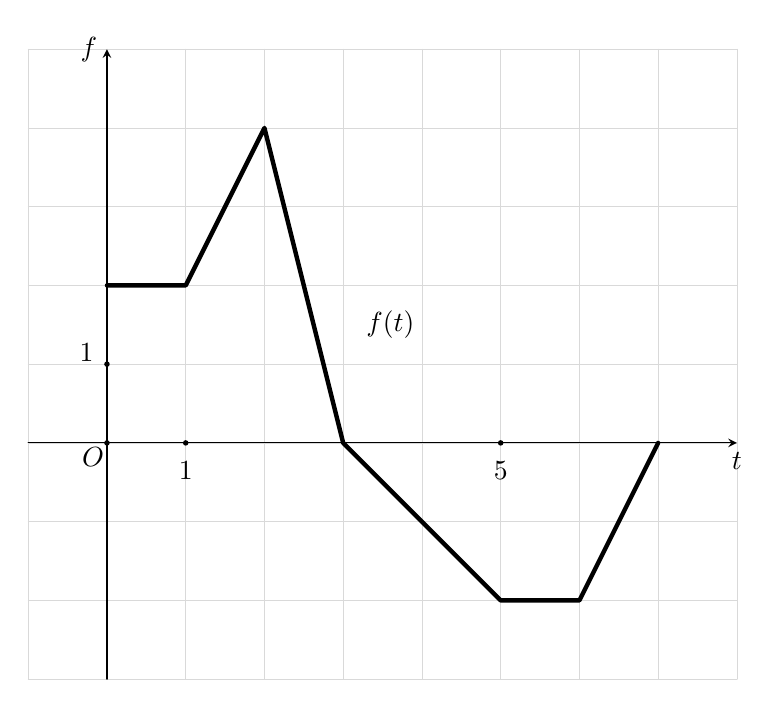
\begin{tikzpicture}[line join=round,line cap=round,>=stealth]
		\draw[step=1,gray!30,very thin] (-1,-3)  grid (8,5);
		\draw[->] (-1,0)--(8,0) node[below]  {$t$};
		\draw[->] (0,-3)--(0,5) node[left]  {$f$};
		\fill (0,0) circle (1pt) node[shift=(-135:0.25)]{$O$}; 
		\foreach \x/\g in {1/-90,5/-90} 
		\fill (\x,0)  circle (1pt) + (\g:3.5mm) node {$\x$};
		 \fill (0,1) circle (1pt) + (150:3mm) node {$1$};
		\draw[ultra  thick] (0,2)--(1,2)--(2,4)--(3,0)--(5,-2)--(6,-2)--(7,0);
		\draw (3.6,1.5)  node{$f (t)$};
	\end{tikzpicture}}}
	\shortans{7} 
	\loigiai{ 
		Ta  có
		$f(t)=\heva{ 
		& 2 &\quad \text{ nếu  } 0\le t\le 1,\\
		&  2t &\quad \text{ nếu } 1\le t\le 2,\\
		&12-4t &\quad \text{ nếu } 2\le t\le 3,\\ 
		& 3-t &\quad \text{  nếu } 3\le t\le 5,\\
		&-2 &\quad \text{ nếu } 5\le t\le  6, \\
		&2t-14 &\quad \text{ nếu } 6\le t\le 7.}$\\ 
		Do đó, 
		\begin{eqnarray*}
			g(3)=\displaystyle\int_0^3 f(t) \mathrm{\,d} t &=&\displaystyle\int_0^1 f(t) \mathrm{\,d} t+\displaystyle\int_1^2 f(t)  \mathrm{\,d} t+\displaystyle\int_2^3 f(t)\mathrm{\,d} t\\
			&=&\displaystyle\int_0^1 2 \mathrm{\,d} t+\displaystyle\int_1^2  2 t \mathrm{\,d} t+\displaystyle\int_2^3(12-4 t) \mathrm{\,d} t \\
			&=&2 t\Big|_0 ^1+t^2\Big|_1 ^2+\left(12 t-2  t^2\right)\Big|_2 ^3=7.
		\end{eqnarray*}
	} 
\end{bt}

% nguồn: Phan2_Lop_12_Dai_so_Chuong_4
\begin{bt}%[2D4V2-2]%[ma:8a0d76e4]
	\immini[thm]{Cho hàm số $y=f(x)$ liên tục trên đoạn $[-3;3]$ có đồ thị như hình vẽ.  Giá trị của tích phân $\displaystyle\int_{-3}^{2}{f(x)}\mathrm{\,d}x$ bằng bao nhiêu? (làm tròn kết quả đến hàng phần mười). }
	{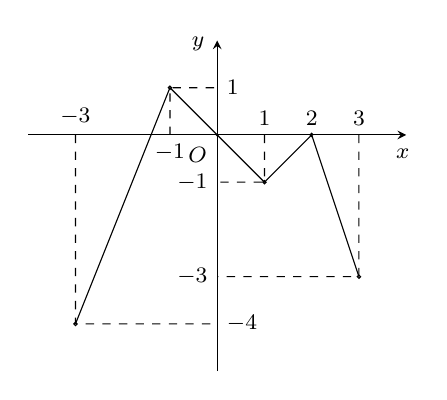
\begin{tikzpicture}[line cap=butt,line join=miter,>=stealth,font=\footnotesize,scale=.6]
		\tikzset{declare  function={xmin=-4; xmax=4; ymin=-5; ymax=2;},
			smooth,samples=450 
		 }
		\draw[->] (xmin,0)--(xmax,0) node[shift={(-100:7pt)}]{$  x $};
		 \draw[->] (0,ymin)--(0,ymax) node[shift={(190:7pt)}]{$ y $};
		\fill (0,0) circle (1pt) node[shift={(225:10pt)}]{$  O $};
		\draw[dashed](-3,0) node[above]{$-3$}|-(0,-4) node[right]{$-4$} 
			(-1,0) node[below]{$-1$}|-(0,1) node[right]{$1$} 
			(1,0) node[above]{$1$}|-(0,-1) node[left]{$-1$} 
			 (2,0) circle (1pt) node[above]{$2$}
			(3,0) node[above]{$3$}|-(0,-3)  node[left]{$-3$};
		\draw (-3,-4) circle  (1pt)
			(-1,1) circle  (1pt)
			 (1,-1) circle (1pt)
			(3,-3) circle  (1pt);
		\draw  (-3,-4)--(-1,1)--(1,-1)--(2,0)--(3,-3);
		\clip (xmin,ymin) rectangle  (xmax,ymax);
	\end{tikzpicture}}
	\shortans{-3,5} 
	\loigiai{ 
		\begin{itemize}
			\item Trên đoạn $[-3;-1]$ đồ thị $f(x)$ là đường thẳng đi qua hai điểm $(-3,-4)$ và $(-1;1)$ nên có phương  trình $f(x)=\dfrac{5}{2}x+\dfrac{7}{2}$.
			\item  Trên đoạn $[-1;1]$ đồ thị $f(x)$ là đường thẳng đi qua hai điểm $(-1,1)$ và $(1;-1)$ nên có phương trình $f(x)=-x$.
			\item Trên đoạn $[1;2]$ đồ thị $f(x)$ là đường thẳng đi qua  hai điểm $(1,-1)$ và $(2;0)$ nên có phương trình $f(x)=x-2$.
		\end{itemize}
		Do  đó
		\begin{align*}
			\displaystyle\int_{-3}^{2}{f(x)}\mathrm{\,d}x=\displaystyle\int_{-3}^{-1}{\left(\dfrac{5}{2}x+\dfrac{7}{2}\right)}\mathrm{\,d}x+\displaystyle\int_{-1}^{1}{(-x)}\mathrm{\,d}x+\displaystyle\int_{1}^{2}{(x-2)}\mathrm{\,d}x=-\dfrac{7}{2}=-3{,}5. 
		\end{align*}
	} 
\end{bt}

% nguồn: Phan2_Lop_12_Dai_so_Chuong_4
\begin{bt}%[2D4V2-2]%[ma:e7e728a5]
	Biết $I=\int_1^3\left|\dfrac{x^2-6x+8}{x+1}\right|\mathrm{\,d}x=\dfrac{a}{b}+c\ln\dfrac{d}{e}$ với $a$ là số nguyên âm  và $b,c,d,e\in\mathbb{Z}^{*}$; $(a,b)=1$, $(d,e)=1$. Giá trị của $a+b+c+d+e$ bằng bao nhiêu?
	\shortans{25} 
	\loigiai{ 
		Ta có $x+1>0$, $\forall x\in[1;3]$, suy ra $\displaystyle\int_1^3\left|\dfrac{x^2-6x+8}{x+1}\right|\mathrm{\,d}x=\int_1^3\dfrac{\left|x^2-6x+8\right|}{x+1}\mathrm{\,d}x$.\\ 
		Ta lại có $x^2-6x+8\leq 0\Leftrightarrow 2\leq x\leq  4$.\\
		Do đó 
		\allowdisplaybreaks\begin{eqnarray*}
		 I&=&\int_1^3\dfrac{\left|x^2-6x+8\right|}{x+1}\mathrm{\,d}x=\int_1^2\dfrac{x^2-6x+8}{x+1}\mathrm{\,d}x-\int_2^3\dfrac{x^2-6x+8}{x+1}\mathrm{\,d}x\\
		&=&\int_1^2\left(x-7+\dfrac{15}{x+1}\right)\mathrm{\,d}x-\int_2^3\left(x-7+\dfrac{15}{x+1}\right)\mathrm{\,d}x\\ 
		&=&\left(-\dfrac{11}{2}+15\ln\dfrac{3}{2}\right)-\left(-\dfrac{9}{2}+15\ln\dfrac{4}{3}\right)\\ 
		&=&-\dfrac{9}{2}+15\ln\dfrac{9}{8}. 
	\end{eqnarray*}
	Vậy $a=-9$, $b=2$, $c=15$, $d=9$, $e=8$ và  $a+b+c+d+e=25$.
} 
\end{bt}

% nguồn: Phan2_Lop_12_Dai_so_Chuong_4
\begin{bt}%[2D4V2-2]%[ma:b1d3de83]
	Cho $0\leq m\leq 2$ và tích phân $I=\int_0^m|x-2|\mathrm{\,d}x=2$. Khi  đó giá trị của tham số $m$ bằng bao nhiêu?
	 \shortans{2}
	 \loigiai{
		Do $x\in[0;m]\Rightarrow  x-2\leq x-m\leq 0\Rightarrow |x-2|=2-x$.\\
		 Khi đó \[I=\int_0^m(2-x)\mathrm{\,d}x=\left(2x-\dfrac{x^2}{2}\right)\bigg|_0^m=2m-\dfrac{m^2}{2}.\]
		Vậy \[I=2\Leftrightarrow 2m-\dfrac{m^2}{2}=2\Leftrightarrow  -m^2+4m-4=0\Leftrightarrow m=2.\]
	 }
\end{bt}


%%%%%%%%%%%%%%%% TỰ LUẬN %%%%%%%%%%%%%%%%

% nguồn: Phan2_Lop_12_Dai_so_Chuong_4
\begin{bt}%[2D4H2-2]%[ma:7ef24878]
	Cho $f(x)=\left\{\begin{array}{ll}1 & \text {khi } x \geq 1 \\ 2 x-1 & \text {khi } x<1
\end{array}\right.$. Tính $J=\displaystyle\int_{-1}^2 f(x) \mathrm{d} x$
 \loigiai{
	 Ta có $
	 J=\displaystyle\int_{-1}^2 f(x) \mathrm{d} x=\displaystyle\int_{-1}^1 f(x) \mathrm{d} x+\displaystyle\int_1^2 f(x) \mathrm{d} x
	 $.\\
	Tính $J_1=\displaystyle\int_{-1}^1 f(x) \mathrm{d} x=\displaystyle\int_{-1}^1(2 x-1) \mathrm{d} x=\left.\left(x^2-x\right)\right|_{-1}^1=0-2=-2$.\\ 
	Tinh $J_2=\displaystyle\int_1^2 f(x) \mathrm{d} x=\displaystyle\int_1^2 1  \mathrm{~d} x=2-1=1$.\\
	Vậy $J=1-2=-1$. 
} 
\end{bt}

% nguồn: Phan2_Lop_12_Dai_so_Chuong_4
\begin{bt}%[2D4H2-2]%[ma:0126d19d]
	Biết rằng $\displaystyle\int_3^4 \dfrac{3x+2}{x^2-3x+2}\mathrm{\,d}x=m\ln 3+n\ln 2$, với $m$, $n\in\mathbb{Z}$. Giá trị của $m+n+2025$  bằng bao nhiêu?
	\loigiai{ 
		Đặt  $\dfrac{3x+2}{(x-1)(x-2)}=\dfrac{A}{x-1}+\dfrac{B}{x-2}\Rightarrow 3x+2=A(x-2)+B(x-1) (A+B)x-2A-B$ (1)\\
		Suy ra  $\heva{&A+B=3\\&2A+B=-2}\Leftrightarrow\heva{&A=-5\\&B=8}$.\\
		Do đó $\dfrac{3x+2}{(x-1)(x-2)}=\dfrac{-5}{x-1}+\dfrac{8}{x-2}$.\\ 
		Ta có 
		\begin{eqnarray*}
			 \displaystyle\int_3^4 &\dfrac{3x+2}{x^2-3x+2}\mathrm{\,d}x&=\displaystyle\int_3^4\left(\dfrac{8}{x-2}-\dfrac{5}{x-1}\right)\mathrm{\,d}x\\
			 &&=\left[8\ln |x-2|-5\ln |x-1|\right]\big|_3^4\\
			 &&=8(\ln 2-\ln 1)-5(\ln 3-\ln 2)\\
			&&=8\ln 2-5\ln 3+5\ln 2\\ 
			&&=13\ln 2-5\ln 3. 
		\end{eqnarray*}
		Suy ra $m=-5$,  $n=13$. Vậy $m+n+2025=-5+13+2025=2033$.
	} 
\end{bt}

% nguồn: Phan2_Lop_12_Dai_so_Chuong_4
\begin{bt}%[2D4V2-2]%[ma:69d3f6c4]
	Tính các  tích phân sau đây.
	\begin{multicols}{2}
		\begin{enumerate}
			\item  $A=\displaystyle\int_{-2}^2\left|x^2-1\right|\mathrm{\,d}x$.
			 \item $B=\displaystyle\int_{-2}^1\left|x^3+x^2-2x\right|\mathrm{\,d}x$.
			\item $C=\displaystyle\int_{-1}^2\left|x^3-3x-2\right|\mathrm{\,d}x$. 
			\item $D=\displaystyle\int_{-2}^2\left|x^4-3x^2-4\right|\mathrm{\,d}x$. 
		\end{enumerate}
	\end{multicols}
	\loigiai{ 
		\begin{enumerate}
			 \item $A=\displaystyle\int_{-2}^2\left|x^2-1\right|\mathrm{\,d}x$.\\
			Xét  $f(x)=x^2-1$ trên đoạn $[-2; 2]$.\\
			Cho $f(x)=0\Leftrightarrow x^2-1=0\Leftrightarrow\hoac{&x=-1\in[-2;  2] \\&x=1\in[-2; 2].}$\\
			Bảng  xét dấu
			\begin{center}
				\begin{tikzpicture}
						\tkzTabInit[nocadre=true,lgt=1.5,espcl=2.5,deltacl=0.5] 
						 {$x$/0.7,$x^2-1$/0.7}
						{$-2$,$-1$,$1$,$2$} 
						\tkzTabLine{,+,0,-,0,+,} 
					\end{tikzpicture}
			\end{center}
			Do đó 
			\begin{eqnarray*}
				 A=\int_{-2}^2\left|x^2-1\right|\mathrm{\,d}x&=&\int_{-2}^{-1}\left(x^2-1\right) \mathrm{\,d}x+\int_{-1}^1\left(1-x^2\right) \mathrm{\,d}x+\int_1^2\left(x^2-1\right) \mathrm{\,d}x\\
				 &=&\left(\dfrac{x^3}{3}-x\right)\bigg|_{-2}^{-1}+\left(x-\dfrac{x^3}{3}\right)\bigg|_{-1}^1+\left(\dfrac{x^3}{3}-x\right)\bigg|_1 ^2\\
				&=&\left[\dfrac{2}{3}-\left(-\dfrac{2}{3}\right)\right]+\left[\dfrac{2}{3}-\left(-\dfrac{2}{3}\right)\right]+\left[\dfrac{2}{3}-\left(-\dfrac{2}{3}\right)\right]\\ 
				 &=&4.
			\end{eqnarray*}
			\item  $B=\displaystyle\int_{-2}^1\left|x^3+x^2-2x\right|\mathrm{\,d}x$.\\
			Xét $f(x)=x^3+x^2-2x$ trên $[-2; 1]$.\\ Cho $f(x)=0\Leftrightarrow  x^3+x^2-2x=0\Leftrightarrow\hoac{&x=-2\in[-2; 1] \\&x=0\in[-2; 1] \\&x=1\in[-2; 1].}$\\
			Bảng xét dấu 
			\begin{center}
				\begin{tikzpicture}
						\tkzTabInit[lgt=1.2,espcl=2.5,nocadre=true] 
						{$x$/0.7,$f (x)$/0.7} 
						 {$-2$,$0$,$1$}
						 \tkzTabLine{0,+,0,-,0,}
					\end{tikzpicture}
			\end{center}
			Do đó 
			\begin{eqnarray*}
				 B&=&\int_{-2}^1\left|x^3+x^2-2x\right|\mathrm{\,d}x\\
				 &=&\int_{-2}^0\left(x^3+x^2-2x\right) \mathrm{\,d}x-\int_0^1\left(x^3+x^2-2x\right) \mathrm{\,d}x\\
				&=&\left.\left(\dfrac{1}{4} x^4+\dfrac{1}{3} x^3-x^2\right)\right|_{-2}^0-\left.\left(\dfrac{1}{4} x^4+\dfrac{1}{3}  x^3-x^2\right)\right|_0 ^1\\
				 &=&-\left(-\dfrac{8}{3}\right)-\left(-\dfrac{5}{12}\right)\\
				 &=&\dfrac{37}{12}.
			\end{eqnarray*}
			\item  $C=\displaystyle\int_{-1}^2\left|x^3-3x-2\right|\mathrm{\,d}x$.\\
			Xét $f(x)=x^3-3x-2$  trên $[-1; 2]$.\\ Cho $f(x)=0\Leftrightarrow x^3-3x-2=0\Leftrightarrow\hoac{&x=2\in[-1; 2] \\&x=-1\in[-1; 2].}$\\
			 Bảng xét dấu
			\begin{center}
				\begin{tikzpicture}
						 \tkzTabInit[lgt=2.5,espcl=2.5,nocadre=true]
						 {$x$/0.7,$x^3-3x-2$/0.7}
						 {$-1$,$2$}
						 \tkzTabLine{0,-,0}
					\end{tikzpicture}
			\end{center}
			Do  đó \[C=-\displaystyle\int_{-1}^2\left(x^3-3x-2\right) \mathrm{\,d}x=-\left.\left(\dfrac{1}{4} x^4-\dfrac{3}{2} x^2-2x\right)\right|_{-1}^2=6-\left(-\dfrac{3}{4}\right)=\dfrac{27}{4}.\]
			 \item $D=\displaystyle\int_{-2}^2\left|x^4-3x^2-4\right|\mathrm{\,d}x$.\\
			Xét $f(x)=x^4-3x^2-4$ trên $[-2; 2]$.\\ 
			Cho  $f(x)=0\Leftrightarrow x^4-3x^2-4=0\Leftrightarrow\hoac{&x=2\in[-2; 2] \\&x=-2\in[-2; 2].}$\\
			Bảng xét dấu 
			\begin{center}
				\begin{tikzpicture}
						 \tkzTabInit[lgt=2.5,espcl=2.5,nocadre=true]
						 {$x$/0.6,$x^4-3x^2-4$/0.6}
						 {$-2$,$2$}
						\tkzTabLine{0,-,0} 
					\end{tikzpicture}
			\end{center}
			Do đó \[D=-\displaystyle\int_{-2}^2\left(x^4-3x^2-4\right)  \mathrm{\,d}x=-\left.\left(\dfrac{1}{5} x^5-x^3-4x\right)\right|_{-2}^2=\dfrac{48}{5}-\left(-\dfrac{48}{5}\right)=\dfrac{96}{5}.\]
		\end{enumerate}
	 }
\end{bt}

% nguồn: Phan2_Lop_12_Dai_so_Chuong_4
\begin{bt}%[2D4V2-2]%[ma:26e14384]
	Tính các tích phân sau đây 
	\begin{multicols}{2}
		\begin{enumerate}
			\item  $A=\displaystyle\int_{-3}^5(|x+2|-|x-2|) \mathrm{\,d}x$.
			\item $B=\displaystyle\int_{-1}^2(x+|1-x|-|x+2|)  \mathrm{\,d}x$.
			\item $C=\displaystyle\int_1^5\dfrac{2|x-2|+1}{x} \mathrm{\,d}x$. 
			 \item $D=\displaystyle\int_0^3\sqrt{x^3-2x^2+x} \mathrm{\,d}x$.
		\end{enumerate}
	\end{multicols}
	\loigiai{ 
		\begin{enumerate}
			 \item $A=\displaystyle\int_{-3}^5(|x+2|-|x-2|) \mathrm{\,d}x$.\\
			Ta có bảng  xét dấu để phá trị tuyệt đối
			\begin{center}
				\begin{tikzpicture}
						\tkzTabInit[lgt=3,espcl=2.5,nocadre=true] 
						 {$x$/0.6,$|x+2|$/0.6,$|x-2|$/0.6,$|x+2|-|x-2|$/0.6}
						 {$-3$,$-2$,$2$,$5$}
						 \tkzTabLine{,-x-2,0,x+2,|,x+2,}
						\tkzTabLine{,-x+2,|,-x+2,0,x-2,} 
						 \tkzTabLine{,-4,|,2x,|,4,}
					\end{tikzpicture}
			\end{center}
			Khi  đó
			\begin{eqnarray*}
				 A&=&\int_{-3}^5\left(|x+2|-|x-2|\right) \mathrm{\,d}x\\
				&=&\int_{-3}^{-2}-4\mathrm{\,d}x+\int_{-2}^22x \mathrm{\,d}x+\int_2^54\mathrm{\,d}x\\ 
				&=&-4x\bigg|_{-3}^{-2}+x^2\bigg|_{-2}^2+4x\bigg|_2  ^5\\
				&=&8. 
			\end{eqnarray*}
			\item $B=\displaystyle\int_{-1}^2(x+|1-x|-|x+2|) \mathrm{\,d}x$.\\ 
			Ta có bảng xét dấu để phá trị tuyệt đối 
			\begin{center}
				\begin{tikzpicture}
						 \tkzTabInit[lgt=3.5,espcl=2.5,nocadre=true]
						 {$x$/0.6,$|1-x|$/0.6,$|x+2|$/0.6,$x+|1-x|-|x+2|$/0.6}
						{$-1$,$1$,$2$} 
						 \tkzTabLine{,1-x,0,x-2,}
						 \tkzTabLine{,x+2,|,x+2,}
						 \tkzTabLine{,-x-1,|,x-3,}
					\end{tikzpicture}
			\end{center}
			Khi đó \begin{eqnarray*}
			 B&=&\int_{-1}^2(x+|1-x|-|x+2|) \mathrm{\,d}x\\
			&=&\int_{-1}^1(-x-1) \mathrm{\,d}x+\int_1^2(x-3)  \mathrm{\,d}x\\
			&=&\left(-\dfrac{x^2}{2}-x\right)\bigg|_{-1}^1+\left(\dfrac{x^2}{2}-3x\right)\bigg|_1 ^2\\ 
			&=&-\dfrac{7}{2}. 
		\end{eqnarray*}
		\item $C=\displaystyle\int_1^5\dfrac{2|x-2|+1}{x}  \mathrm{\,d}x$.\\
		 Ta có $|x-2|=\heva{&x-2&\text{ khi } x \geq 2\\-&x+2&\text{ khi } x < 2.}$\\
		Khi  đó
		\begin{eqnarray*}
			C=\int_1^5\dfrac{2|x-2|+1}{x} \mathrm{\,d}x&=&\int_1^2\dfrac{2(2-x)+1}{x} \mathrm{\,d}x+\int_2^5\dfrac{2(x-2)+1}{x}  \mathrm{\,d}x\\
			&=&\int_1^2\dfrac{5-2x}{x} \mathrm{\,d}x+\int_2^5\dfrac{2x-3}{x}  \mathrm{\,d}x\\
			&=&\int_1^2\left(\dfrac{5}{x}-x\right) \mathrm{\,d}x+\int_2^5\left(2-\dfrac{3}{x}\right) \mathrm{\,d}x\\ 
			 &=&\left(5\ln|x|-x\right)\bigg|_1 ^2+\left(2x-3\ln|x|\right)\bigg|_2 ^5\\
			&=&8\ln 2-3\ln 5+4. 
		\end{eqnarray*}
		\item $D=\displaystyle\int_0^3\sqrt{x^3-2x^2+x} \mathrm{\,d}x$.\\ 
		Ta  có $D=\displaystyle\int_0^3\sqrt{x^3-2x^2+x} \mathrm{\,d}x=\int_0^3\sqrt{x\left(x^2-2x+1\right)} \mathrm{\,d}x=\int_0^3|x-1|\sqrt{x} \mathrm{\,d}x$.\\
		 Lại có $|x-1|=\heva{&x-1&\text{ khi } x \geq 1\\-&x+1&\text{ khi } x < 1.}$\\
		 Khi đó
		\begin{eqnarray*}
			D&=&\int_0^3(1-x)  \sqrt{x} \mathrm{\,d}x+\int_0^3(x-1) \sqrt{x} \mathrm{\,d}x\\
			&=&\int_0^3\left(x^{\tfrac{1}{2}}-x^{\tfrac{3}{2}}\right) \mathrm{\,d}x+\int_0^3\left(x^{\tfrac{3}{2}}-x^{\tfrac{1}{2}}\right)  \mathrm{\,d}x\\
			&=&\left(\dfrac{2}{3}  x \sqrt{x}-\dfrac{2}{5} x^2\sqrt{x}\right)\bigg|_0 ^1+\left(\dfrac{2}{5} x^2\sqrt{x}-\dfrac{2}{3} x \sqrt{x}\right)\bigg|_1 ^3\\
			 &=&\dfrac{4}{15}+\left[\dfrac{8\sqrt{3}}{5}-\left(-\dfrac{4}{15}\right)\right]\\
			&=&\dfrac{24\sqrt{3}+8}{15}. 
		\end{eqnarray*}
	\end{enumerate}
 }
\end{bt}
